% ==============================================================================
% BÁO CÁO VỀ DỮ LIỆU -- Nhóm 11, CSC14005, FIT HCMUS
% Biên dịch bằng XeLaTeX: sh make.sh  (hoặc xem README.md trong thư mục này)
% Dùng lại fit_hcmus.sty và logo của đề cương (../proposal/latex/).
% ==============================================================================
\documentclass[12pt,a4paper]{article}
\usepackage{scrextend}
\changefontsizes{13pt}

\makeatletter
\def\input@path{{../proposal/latex/}}
\makeatother
\usepackage{fit_hcmus}
\usepackage{longtable}
\usepackage{needspace}
\usepackage{multirow}
\usepackage{subcaption}
\graphicspath{{../proposal/latex/}{figures_vi/}{figures/}}
\setlength{\emergencystretch}{3em}

% ---------------------------------------------------------------- thông tin
\courseid{CSC14005}
\coursename{Nhập môn Học máy}
\reportsubtitle{BÁO CÁO VỀ DỮ LIỆU}
\title{PHÂN LOẠI TÌNH TRẠNG CHẶN LỐI ĐI TRÊN VỈA HÈ TP.HCM TỪ ẢNH ĐƯỜNG PHỐ}
\instructor{TS. Bùi Tiến Lên}
\classid{24KHMT02}
\academicyear{Học kỳ I, năm học 2026 - 2027}
\groupid{11}
\author{
    \renewcommand{\arraystretch}{1.1}
    \begin{tabular}{cc}
        \textbf{Họ và tên} & \textbf{MSSV} \\
        Lê Nguyễn Quốc Học & 24127044 \\
        Bùi Thị Bích Loan & 24127072 \\
        Nguyễn Hữu Gia Minh & 24127078 \\
        Nguyễn Lê Hoàng Khải & 24127408 \\
        Trần Hoàng Phúc & 24127505
    \end{tabular}
}

% ---------------------------------------------------------------- tiếng Việt cho khung của fit_hcmus.sty
\makeatletter
\renewcommand{\tableofcontents}{\fit@listheading{Mục lục}\@starttoc{toc}}
\renewcommand{\listoftables}{\vspace{14pt}\fit@listheading{Danh sách bảng}\@starttoc{lot}}
\renewcommand{\listoffigures}{\vspace{14pt}\fit@listheading{Danh sách hình}\@starttoc{lof}}
\titlecontents{figure}[3.8em]{}{\contentslabel{2.3em}}{}{\titlerule*[0.75em]{.}\contentspage}
\renewcommand{\refname}{Tài liệu tham khảo}
\renewcommand{\figurename}{Hình}
\renewcommand{\tablename}{Bảng}
\fancypagestyle{fancy}{%
  \fancyhf{}%
  \fancyhead[L]{\small\bfseries\color{fitdark}\@courseid: \@coursename}%
  \fancyhead[R]{\small\bfseries\color{fitprimary}Khoa CNTT, ĐH KHTN TP.HCM}%
  \fancyfoot[L]{\small\itshape\color{fitgray}Báo cáo về dữ liệu -- Nhóm \@groupid}%
  \fancyfoot[R]{\small\bfseries\color{fitdark}Trang \thepage/\pageref{LastPage}}%
  \renewcommand{\headrulewidth}{0.6pt}%
  \renewcommand{\footrulewidth}{0.5pt}%
  \renewcommand{\footruleskip}{12.4pt}%
}
\fancypagestyle{plain}{%
  \fancyhf{}%
  \fancyfoot[R]{\raisebox{8pt}[0pt][0pt]{\small\bfseries\color{fitdark}Trang \thepage}}%
  \renewcommand{\headrulewidth}{0pt}%
  \renewcommand{\footrulewidth}{0pt}%
}
\renewcommand{\makecoverpage}{%
  \begin{titlepage}
  \setstretch{1.0}%
  \centering
  \vspace*{\dimexpr-0.9cm+3bp\relax}
  \begin{adjustwidth}{-0.5cm}{0.5cm}
  \centering
  {\fontsize{13pt}{16pt}\selectfont\bfseries ĐẠI HỌC QUỐC GIA THÀNH PHỐ HỒ CHÍ MINH\par}
  \vspace{4.2pt}
  {\fontsize{14pt}{16pt}\selectfont\bfseries\color{fitprimary} TRƯỜNG ĐẠI HỌC KHOA HỌC TỰ NHIÊN\par}
  \vspace{1.9pt}
  {\fontsize{13pt}{16pt}\selectfont\bfseries\color{fitaccent} KHOA CÔNG NGHỆ THÔNG TIN\par}
  \vspace{8.3pt}
  {\color{fitaccent}\rule{10.4cm}{1.5pt}\par}
  \vspace{16.9pt}
  
\includegraphics[width=4.4cm]{images/logo_hcmus.png}\par
  \vspace{22.8pt}
  {\fontsize{13pt}{16pt}\selectfont\bfseries MÔN HỌC: \@coursename\ (\@courseid)\par}
  \vspace{5pt}
  {\fontsize{14pt}{16pt}\selectfont\bfseries\color{fitdark}\@reportsubtitle\par}
  \vspace{8.1pt}
  \begin{tcolorbox}[enhanced,width=\linewidth,arc=5.5pt,boxrule=1.5pt,
      colframe=fitprimary,colback=white,halign=center,valign=center,
      top=12pt,bottom=12pt,left=8pt,right=8pt]
    \fontsize{17pt}{21pt}\selectfont\bfseries\color{fitprimary}\@title
  \end{tcolorbox}
  \vspace{-2.1pt}
  {\fontsize{13pt}{16pt}\selectfont
   \renewcommand{\arraystretch}{1.7}%
   \begin{tabular}{@{}l@{\hspace{1.2em}}l@{}}
     \textbf{Giảng viên:} & \@instructor \\
     \textbf{Lớp:} & \@classid \\
     \textbf{Thời gian:} & \@academicyear \\
     \textbf{Nhóm:} & \@groupid \\
     \textbf{Sinh viên:} &
   \end{tabular}\par}
  \vspace{2pt}
  {\fontsize{13pt}{16pt}\selectfont\setstretch{1.35}\@author\par}
  \end{adjustwidth}
  \vfill
  \end{titlepage}%
}
\makeatother

% ---------------------------------------------------------------- lệnh riêng của báo cáo
% \note{...}: ghi chú cách tính, in nhỏ và xám ngay dưới bảng/đoạn văn.
\newcommand{\note}[1]{{\par\noindent\footnotesize\color{fitgray}\textit{Ghi chú:} #1\par}}
\newcommand{\f}[1]{\path{#1}}                      % đường dẫn file, cho phép ngắt dòng
\newcommand{\lab}[1]{\textsf{#1}}                  % tên nhãn, tên cột
\newcommand{\cc}{© Mapillary contributors, CC BY-SA 4.0}
\newcolumntype{R}{>{\raggedleft\arraybackslash}X}
\newcolumntype{C}{>{\centering\arraybackslash}X}

\begin{document}

\makecoverpage
\pagestyle{plain}
\pagenumbering{roman}
\begingroup
    \setstretch{1.0}
    \setlength{\parskip}{0pt}
    \small
    \tableofcontents
    \vspace{1.5em}
    \listoftables
    \vspace{0.5em}
    \listoffigures
\endgroup
\newpage
\pagestyle{fancy}
\pagenumbering{arabic}
\small

% ==============================================================================
% 1. GIỚI THIỆU BÀI TOÁN
% ==============================================================================
\section{Giới thiệu bài toán}

\subsection{Bài toán học máy}

Một vỉa hè có thể tồn tại về mặt vật lý nhưng không còn đóng vai trò lối đi bộ khi xe đậu, hàng hóa, bàn ghế hoặc rào chắn làm gián đoạn lối đi liên tục. Đồ án xây dựng một bộ phân loại ảnh nhằm sàng lọc tình trạng này trên ảnh đường phố tại TP.HCM.

\begin{itemize}
  \item \textbf{Đầu vào:} một ảnh $640\times640$ điểm ảnh nhìn về một phía vỉa hè, được cắt từ ảnh toàn cảnh $360^\circ$ chụp từ xe.
  \item \textbf{Đầu ra của mô hình:} phân loại nhị phân. \lab{0 -- Còn lối đi}: người đi bộ có thể tiếp tục đi dọc vỉa hè gần. \lab{1 -- Bị chặn}: người đi bộ buộc phải bước xuống lòng đường.
  \item \textbf{Ảnh không đủ bằng chứng} (không thấy vỉa hè gần, bị che khuất, ảnh hỏng) được gán nhãn riêng \lab{I -- Không đủ thông tin}; nhãn này chỉ dùng ở khâu gán nhãn và các ảnh mang nhãn \lab{I} bị loại khỏi quá trình huấn luyện và đánh giá mô hình. Nhãn \lab{I} vẫn được thống kê vì nó quyết định số ảnh hợp lệ thu được từ nguồn dữ liệu.
  \item \textbf{Câu hỏi nghiên cứu:} mô hình nào phân loại tốt nhất trên \emph{các tuyến đường không xuất hiện trong tập huấn luyện}. Do đó, dữ liệu được chia theo nguyên tuyến đường, và mọi kiểm tra trong báo cáo đều chú trọng tới rò rỉ dữ liệu giữa các tập.
\end{itemize}

Với mỗi ảnh, người gán nhãn trả lời câu hỏi: \emph{người đi bộ có phải bước xuống lòng đường để tiếp tục đi dọc vỉa hè gần không?}

\textbf{Quy ước thuật ngữ.} Báo cáo dùng tên viết tắt train, val và test cho tập huấn luyện, tập kiểm định và tập kiểm thử. \emph{Ảnh hợp lệ} là ảnh có nhãn \lab{0} hoặc \lab{1}; \emph{mẫu dương} là ảnh có nhãn \lab{Bị chặn}. \emph{Metadata} (siêu dữ liệu) là các thuộc tính đi kèm mỗi ảnh như tọa độ, thời gian chụp và tài khoản chụp. EDA là viết tắt của phân tích khám phá dữ liệu (exploratory data analysis). Thành viên nhóm được gọi theo tên: Học (Lê Nguyễn Quốc Học), Loan (Bùi Thị Bích Loan), Minh (Nguyễn Hữu Gia Minh), Khải (Nguyễn Lê Hoàng Khải) và Phúc (Trần Hoàng Phúc).

\subsection{Tổng quan bộ dữ liệu}

Bộ dữ liệu gồm ba phần, được thu thập theo ba cách lấy mẫu khác nhau (bảng~\ref{tab:overview}). Báo cáo luôn trình bày tách riêng ba phần này, vì chỉ phần thứ nhất phản ánh phân phối tự nhiên của ảnh trên các tuyến đường.

\begin{table}[H]
\centering
\caption{Ba phần của bộ dữ liệu và nhãn cuối (đơn vị: ảnh)}
\label{tab:overview}
\begin{tabularx}{\textwidth}{>{\raggedright\arraybackslash}p{0.27\linewidth}L r r r r}
\toprule
\textbf{Phần} & \textbf{Cách lấy mẫu} & \textbf{Ảnh} & \textbf{0} & \textbf{1} & \textbf{I} \\
\midrule
Bộ chính, train & Tự nhiên: mọi vị trí cách nhau 25 m trên 10 đường & 1.839 & 939 & 106 & 794 \\
Bộ chính, val & Tự nhiên, 3 đường & 486 & 207 & 35 & 244 \\
Bộ chính, test & Tự nhiên, 4 đường & 674 & 412 & 47 & 215 \\
Pilot, train & Theo tầng điểm của một mô hình thử, 3 đường train & 150 & 73 & 14 & 63 \\
Ảnh bổ sung, train & 70\% theo điểm của bộ chọn ảnh, 30\% ngẫu nhiên, 75 đường mới & 2.000 & 819 & 577 & 604 \\
\midrule
\textbf{Tổng} & & \textbf{5.149} & \textbf{2.450} & \textbf{779} & \textbf{1.920} \\
\bottomrule
\end{tabularx}
\end{table}

Một số lưu ý khi đọc các phần tiếp theo:
\begin{itemize}
  \item \textbf{Val và test chỉ gồm ảnh tự nhiên.} Ảnh pilot và ảnh bổ sung chỉ được đưa vào train. Nhãn val/test chỉ dùng để thống kê mô tả, không dùng để lựa chọn hay điều chỉnh bất kỳ thành phần nào.
  \item \textbf{Lớp \lab{Bị chặn} hiếm trong ảnh tự nhiên:} 188 trên 1.746 ảnh hợp lệ của bộ chính (10,8\%). Đây là lý do nhóm thực hiện đợt bổ sung ảnh cho train.
  \item \textbf{Khoảng 40\% ảnh mang nhãn \lab{Không đủ thông tin}}, do ảnh chụp từ xe thường không quan sát rõ vỉa hè gần.
\end{itemize}

% ==============================================================================
% 2. PHƯƠNG PHÁP VÀ NGUỒN THU THẬP DỮ LIỆU
% ==============================================================================
\needspace{0.5\textheight}
\section{Phương pháp và nguồn thu thập dữ liệu}

\subsection{Nguồn dữ liệu}

Bảng~\ref{tab:sources} lần lượt trả lời các câu hỏi về nguồn dữ liệu trong khung báo cáo.

\begin{table}[H]
\centering
\caption{Trả lời các câu hỏi về nguồn dữ liệu của khung báo cáo}
\label{tab:sources}
\begin{tabularx}{\textwidth}{>{\raggedright\arraybackslash}p{0.27\linewidth}L}
\toprule
\textbf{Câu hỏi} & \textbf{Trả lời} \\
\midrule
Dựa trên dataset có sẵn? & Không. Nhóm tự xây dựng bộ dữ liệu từ ảnh gốc. Bộ dữ liệu gần nhất là Vietnamese Sidewalk Violation VQA~\cite{dao2026viahevqa}, nhưng bộ này không có tọa độ và thời gian chụp nên không thể chia theo tuyến đường; nhóm không sử dụng ảnh hay nhãn của bộ này. \\
Từ API? & Có. Ảnh $360^\circ$ và metadata được lấy qua Mapillary Graph API~\cite{mapillary2024intro}; mạng lưới đường và các điểm ngữ cảnh (chợ, trường học) được lấy từ OpenStreetMap (OSM)~\cite{osm2026} qua Overpass API. \\
Web scraping? & Không. \\
Khảo sát, biểu mẫu? & Không. Nhãn do 5 thành viên nhóm gán trên Label Studio~\cite{labelstudio2020} (mục~\ref{sec:labeling}). \\
Giấy phép & Ảnh Mapillary theo giấy phép CC BY-SA 4.0, ghi công \cc. Phần làm mờ khuôn mặt và biển số của Mapillary được giữ nguyên. Ảnh không được đưa lên git. \\
Ảnh nhóm tự chụp & \textbf{Chưa có} (đề cương dự kiến ít nhất 100 ảnh). \\
\bottomrule
\end{tabularx}
\end{table}

Khu vực nghiên cứu là trung tâm TP.HCM (Quận 1, 3, 5, 10, Phú Nhuận và Bình Thạnh cũ), trong khung tọa độ 10,745--10,815$^\circ$ Bắc, 106,650--106,725$^\circ$ Đông. Trong khung này, Mapillary có 652.159 ảnh $360^\circ$ thuộc 1.234 chuỗi ảnh (quét ngày 22/10/2026), chủ yếu của ba tài khoản \lab{bemaps3\_sg}, \lab{phoenix\_mapping\_front} và \lab{phoenixmap\_front}, chụp trong các năm 2016, 2023 và 2024.

\subsection{Quy trình thu thập từng bước}
\label{sec:pipeline}

Bảng~\ref{tab:steps} liệt kê chín bước thu thập và kết quả của từng bước. Mỗi bước do một script riêng của nhóm thực hiện và được ghi lại trong nhật ký thu thập.

\begin{table}[H]
\centering
\caption{Các bước thu thập bộ chính và pilot}
\label{tab:steps}
\begin{tabularx}{\textwidth}{c >{\raggedright\arraybackslash}p{0.34\linewidth} L}
\toprule
\textbf{\#} & \textbf{Công việc} & \textbf{Kết quả} \\
\midrule
1 & Lấy các đường có tên và các điểm ngữ cảnh từ OSM & 7.283 đoạn đường, 6.715 điểm \\
2 & Quét metadata ảnh $360^\circ$ theo các ô lưới 0,001$^\circ$ & 652.159 ảnh; 2 ô nhỏ ở góc khung bị lỗi \\
3 & Gắn ảnh vào đường: cách đường $\le 20$ m và hướng di chuyển lệch trục đường $\le 30^\circ$; loại hẻm & 81,3\% số ảnh gắn được vào một đường \\
4 & Xem trước 56 đường, mỗi đường 20 vị trí, để chọn đường & Loại 7 đường ven kênh, cầu, đường hầm; chọn 17 đường \\
5 & Chia 17 đường thành train/val/test \emph{trước khi} gán nhãn & 10 đường train, 3 đường val, 4 đường test \\
6 & Pilot: 150 ảnh trên 3 đường train, cả 5 người cùng gán mỗi ảnh & Fleiss $\kappa$~\cite{fleiss1971kappa} 0,57; viết lại hướng dẫn gán nhãn (v1) \\
7 & Thu thập bộ chính: các vị trí cách nhau 25 m, tối đa 2 ảnh mỗi vị trí từ hai ngày khác nhau, tối đa 420 ảnh mỗi đường, bỏ các vị trí của pilot & Chọn 3.057 ảnh, loại 58 ảnh chụp ban đêm, còn 2.999 ảnh \\
8 & Gán nhãn bộ chính, đo đồng thuận, phân xử (mục~\ref{sec:labeling}) & Nhãn cuối cho 3.149 ảnh \\
9 & Bổ sung ảnh cho train từ 75 đường mới (mục~\ref{sec:enrich}) & 2.000 ảnh, trong đó 577 ảnh \lab{Bị chặn} \\
\bottomrule
\end{tabularx}
\end{table}

\textbf{Cắt ảnh.} Mỗi ảnh $360^\circ$ cho đúng một ảnh cắt: nhìn về bên phải xe, lệch $60^\circ$ so với hướng di chuyển (góc yaw), nghiêng xuống $4^\circ$ (góc pitch), trường nhìn $90^\circ$, kích thước $640\times640$ điểm ảnh, lưu dạng JPEG chất lượng 90. Hai quyết định dưới đây dựa trên phép đo thăm dò ngày 23/10/2026, không dựa trên nhãn:
\begin{itemize}
  \item \emph{Chỉ cắt ảnh bên phải.} Trên 1.166 ảnh $360^\circ$, một phép đo tự động (với tiêu chí chặt) phát hiện vỉa hè gần ở 38\% ảnh bên phải và 7\% ảnh bên trái. Ảnh bên trái phần lớn chỉ thấy lòng đường, dải phân cách hoặc vỉa hè phía đối diện. Hệ quả là vỉa hè bên trái của đường một chiều ít được quan sát.
  \item \emph{Góc lệch $60^\circ$ và góc nghiêng $4^\circ$} cho tỉ lệ quan sát được vỉa hè gần cao nhất trong 6 tổ hợp đã thử (góc lệch 60/75/90$^\circ$, góc nghiêng 4/10$^\circ$).
\end{itemize}

\textbf{Chia tập theo tuyến đường.} Mỗi đường thuộc trọn một tập, nhờ đó mô hình được đánh giá trên các đường chưa từng thấy. Bốn đường test nằm ở bốn khu vực khác nhau. Danh sách đường và tập được xác định ngày 23/10/2026, trước khi có bất kỳ nhãn nào của bộ chính. Hiện việc chia tập đã hoàn tất nhưng \emph{chưa được khóa}, do nhóm còn chờ quyết định cách xử lý các ảnh train nằm gần giao lộ với val/test. Nhóm giữ nguyên các đường test đã định: việc test chỉ có 47 mẫu dương là một hạn chế về độ chính xác của đánh giá, không phải tiêu chí để thay đổi tập dựa trên nhãn đã quan sát.

\subsection{Gán nhãn}
\label{sec:labeling}

Nhãn do người gán, theo hướng dẫn gán nhãn phiên bản v1 (bản đã được nhóm thống nhất nguyên văn). Mỗi ảnh được xét qua ba câu hỏi theo thứ tự:
\begin{enumerate}
  \item Ảnh có quan sát được không? Ảnh mờ, tối hoặc cháy sáng đến mức không thể đánh giá thì gán \lab{I}.
  \item Có thấy vỉa hè gần không? Phải có một đoạn mép vỉa hè nằm dưới vạch 3/5 chiều cao ảnh; nếu không (chỉ thấy lòng đường, vỉa hè ở xa, giao lộ, đầu hẻm, hoặc bị che quá nửa) thì gán \lab{I}.
  \item Lối đi có liên tục không? Nếu không thể đi thẳng qua thì gán \lab{1}. Người và xe đang di chuyển không được tính là vật cản; chỉ xét vật cản trong phạm vi tới khoảng giữa ảnh.
\end{enumerate}

Ngoài nhãn chính, người gán ghi lý do khi chọn \lab{I} (4 lý do), có thể đánh dấu loại vật cản (6 loại, không bắt buộc), ô \lab{Khó / không chắc} và ghi chú tự do. Giao diện gán nhãn trên Label Studio được cấu hình theo đúng ba câu hỏi trên.

\begin{table}[H]
\centering
\caption{Phân công gán nhãn}
\label{tab:assignment}
\begin{tabularx}{\textwidth}{>{\raggedright\arraybackslash}p{0.22\linewidth} r L}
\toprule
\textbf{Phần} & \textbf{Ảnh} & \textbf{Cách gán} \\
\midrule
Test & 674 & Hai người (Học, Loan) gán độc lập mọi ảnh \\
Val & 486 & Hai người (Minh, Khải) gán độc lập mọi ảnh \\
Train, bộ chính & 1.839 & Mỗi ảnh một người; 276 ảnh (15\%) được người thứ hai gán chéo \\
Pilot & 150 & 5 người gán theo hướng dẫn v0; sau đó cả 150 ảnh được xem lại theo v1 \\
Ảnh bổ sung & 2.000 & Mỗi ảnh một người (5 người, mỗi người 400 ảnh được chia ngẫu nhiên); 203 ảnh được người thứ hai kiểm tra chéo \\
\bottomrule
\end{tabularx}
\end{table}

Bảng~\ref{tab:assignment} cho biết phân công gán nhãn. Người gán không thấy tên đường, tập dữ liệu, điểm của mô hình hay phiếu của người khác. Ảnh của các tập được trộn lẫn trong cùng một dự án gán nhãn. Bộ chính có tổng cộng $5\times887 = 4.435$ lượt gán, không thiếu lượt nào. Kết quả đồng thuận và phân xử được trình bày ở mục~\ref{sec:qa}.

\subsection{Bổ sung mẫu dương cho train}
\label{sec:enrich}

Sau đợt gán nhãn đầu tiên, train chỉ có 120 mẫu dương (gồm 14 ảnh pilot). Nhóm bổ sung ảnh \emph{chỉ vào train}, theo hướng chủ động tìm mẫu dương của lớp hiếm~\cite{attenberg2010search}:

\begin{enumerate}
  \item \textbf{Bộ chọn ảnh.} Hồi quy logistic trên vector đặc trưng (embedding) DINOv2 ViT-B/14~\cite{oquab2023dinov2}, huấn luyện trên 1.989 nhãn train (120 mẫu dương). Bộ chọn này được lựa chọn qua một phép so sánh chỉ dùng nhãn train, theo cách để riêng từng tuyến đường (leave-one-street-out): trong 20\% ảnh có điểm cao nhất có 22,0\% ảnh \lab{Bị chặn}, so với 13,9\% của bộ chấm điểm cũ (chênh lệch $+8{,}2$ điểm phần trăm, khoảng tin cậy 95\% $[4{,}3;\,11{,}7]$) và 5,8\% nếu lấy mẫu ngẫu nhiên.
  \item \textbf{Chọn đường.} Quét 150 đường chưa sử dụng (mỗi đường 30 ảnh), xếp hạng theo điểm trung bình và lấy 75 đường đứng đầu. Đường trùng tên với đường val/test bị loại, kể cả các đoạn khác của cùng đường.
  \item \textbf{Chọn ảnh.} Kho ứng viên gồm 5.035 ảnh. Nhóm chọn 2.000 ảnh: 1.400 ảnh có điểm cao nhất (\emph{tầng điểm cao}, điểm $\ge 0{,}61$) và 600 ảnh lấy ngẫu nhiên trong phần còn lại (\emph{tầng ngẫu nhiên}). Các vị trí cách ảnh val/test dưới 40 m bị loại.
  \item \textbf{Gán nhãn.} Giống phần train của bộ chính, mỗi ảnh do một người gán; người gán không biết ảnh thuộc tầng nào.
\end{enumerate}

Điểm của bộ chọn ảnh \emph{chỉ dùng để chọn ảnh cho người gán, không bao giờ được dùng làm nhãn}. Vì ảnh bổ sung được chọn có chủ đích, phân phối của chúng lệch khỏi phân phối tự nhiên~\cite{farquhar2021bias}. Tầng ngẫu nhiên (30\%) được lấy từ phần còn lại sau khi chọn tầng điểm cao, nên không phải là mẫu ngẫu nhiên vô điều kiện của toàn kho ứng viên; tầng này được giữ để so sánh hiệu suất thu được mẫu dương trên đường mới. Mọi thống kê trong báo cáo đều tách ảnh bổ sung khỏi bộ chính.

\subsection{Công cụ và định dạng lưu trữ}

Bảng~\ref{tab:tools} tóm tắt công cụ và định dạng lưu trữ ở từng bước; vị trí lưu từng loại dữ liệu được trình bày ở mục~\ref{sec:storage}.

\begin{table}[H]
\centering
\caption{Công cụ sử dụng và định dạng lưu trữ}
\label{tab:tools}
\begin{tabularx}{\textwidth}{>{\raggedright\arraybackslash}p{0.25\linewidth} >{\raggedright\arraybackslash}p{0.30\linewidth} L}
\toprule
\textbf{Công việc} & \textbf{Công cụ} & \textbf{Định dạng lưu} \\
\midrule
Mạng lưới đường, điểm ngữ cảnh & Overpass API, shapely & JSON \\
Metadata ảnh & Mapillary Graph API, requests, pandas & Parquet \\
Ảnh $360^\circ$ gốc & Mapillary (ảnh thu nhỏ 2.048 điểm ảnh) & JPEG \\
Cắt ảnh & py360convert, Pillow & JPEG $640\times640$ \\
Danh mục ảnh (manifest) & pandas & CSV UTF-8, mỗi ảnh một dòng \\
Gán nhãn & Label Studio tự triển khai trên AWS (Docker, Caddy) & Export JSON trên server; bảng nhãn CSV trong repo \\
Đo đồng thuận, thống kê & pandas, SciPy, scikit-learn & CSV, Markdown \\
Bộ chọn ảnh, đo độ phủ vỉa hè (chỉ phục vụ chọn mẫu) & PyTorch, Transformers (DINOv2~\cite{oquab2023dinov2}, CLIP~\cite{radford2021clip}, SegFormer~\cite{xie2021segformer}) & Embedding NPZ \\
Cấu hình đường và tập & & YAML \\
EDA của báo cáo này & pandas, SciPy, Matplotlib & CSV, JSON, PDF, JPEG \\
\bottomrule
\end{tabularx}
\end{table}

% ==============================================================================
% 3. LÀM SẠCH, TIỀN XỬ LÝ, ĐẢM BẢO CHẤT LƯỢNG, LƯU TRỮ
% ==============================================================================
\needspace{0.3\textheight}
\section{Quy trình làm sạch và tiền xử lý dữ liệu}
\label{sec:cleaning}

Nguyên tắc chung của nhóm là \emph{chỉ lọc dữ liệu bằng quy tắc, không lọc bằng mô hình}, và không chỉnh sửa dữ liệu gốc. Bảng~\ref{tab:cleaning} trình bày từng bước làm sạch, cách thực hiện và số lượng ảnh bị loại.

\begin{longtable}{>{\raggedright\arraybackslash}p{0.21\linewidth} >{\raggedright\arraybackslash}p{0.44\linewidth} >{\raggedright\arraybackslash}p{0.26\linewidth}}
\caption{Các bước làm sạch và tiền xử lý, theo khung báo cáo}
\label{tab:cleaning}\\
\toprule
\textbf{Nội dung} & \textbf{Cách thực hiện} & \textbf{Kết quả} \\
\midrule
\endfirsthead
\toprule
\textbf{Nội dung} & \textbf{Cách thực hiện} & \textbf{Kết quả} \\
\midrule
\endhead
Ảnh chụp ban đêm & Loại ảnh có độ sáng trung bình nửa trên của ảnh $360^\circ$ dưới 90 (thang 0--255). Không lọc theo giờ chụp vì giờ ghi trên Mapillary không đáng tin cậy (nhiều ảnh ghi 18--0 giờ vẫn sáng như ban ngày). & Bộ chính: loại 58/3.057. Kho ứng viên bổ sung: loại 38/5.074 \\
Ảnh không thuộc tuyến đường & Chỉ giữ ảnh cách đường $\le 20$ m và có hướng di chuyển dọc trục đường ($\le 30^\circ$); loại hẻm. & 81,3\% ảnh trong khu vực gắn được vào đường \\
Ảnh không đủ thông tin & Không lọc tự động. Người gán đặt nhãn \lab{I} kèm lý do; ảnh \lab{I} bị loại khỏi mô hình nhưng vẫn được giữ trong bảng nhãn. & 1.920/5.149 ảnh mang nhãn \lab{I} \\
Trùng lặp tuyệt đối & Mỗi ảnh $360^\circ$ chỉ được dùng một lần; so sánh mã băm MD5 của ảnh cắt. & Xem mục~\ref{sec:eda-quality} \\
Gần trùng & Lấy mẫu thưa: mỗi 25 m một vị trí, tối đa 2 ảnh mỗi vị trí và phải khác ngày chụp. Riêng kho ứng viên bổ sung có thêm bước so sánh mã băm sai phân (dHash)~\cite{krawetz2013dhash} giữa hai ngày chụp của cùng vị trí. & Kho ứng viên bổ sung: loại 1 cặp. Bộ chính: được đánh giá lần đầu trong báo cáo này (mục~\ref{sec:eda-quality}) \\
Dữ liệu thiếu & Metadata lấy từ API; ảnh thiếu tọa độ hoặc hướng di chuyển không gắn được vào đường nên đã bị loại ở bước gắn đường. Với nhãn, mọi lượt gán đều bắt buộc chọn nhãn chính. & Xem bảng~\ref{tab:inventory} \\
Chuẩn hóa, biến đổi & Chiếu ảnh $360^\circ$ về ảnh phối cảnh $640\times640$ điểm ảnh với cùng tham số cho mọi ảnh (mục~\ref{sec:pipeline}). Chưa chuẩn hóa giá trị điểm ảnh; bước này thuộc giai đoạn huấn luyện. & Mọi ảnh có cùng kích thước và góc nhìn \\
Chuyển đổi kiểu dữ liệu & Nhãn Label Studio (chuỗi tiếng Việt) $\rightarrow$ mã \lab{0}/\lab{1}/\lab{I}. Mã ảnh $360^\circ$ (số 64 bit) $\rightarrow$ mã ảnh 8 ký tự không để lộ nguồn cho người gán. Thời gian chụp được giữ dạng chuỗi ISO có múi giờ. & Áp dụng thống nhất cho mọi bảng nhãn của bộ chính, pilot và ảnh bổ sung \\
Kiểm tra nhất quán & Bước thu thập từ chối các đường đã thuộc tập khác; báo cáo này kiểm tra lại toàn bộ khóa, tập, đường và tọa độ. & Mục~\ref{sec:eda-quality} \\
\bottomrule
\end{longtable}

\textbf{Các việc chưa thực hiện:} rà soát nội dung nhạy cảm trong ảnh (ngoài phần làm mờ sẵn của Mapillary) và khóa danh sách chia tập.

% ------------------------------------------------------------------------------
\needspace{0.45\textheight}
\section{Đảm bảo chất lượng dữ liệu}
\label{sec:qa}

\subsection{Tiêu chí dữ liệu tốt cho bài toán này}

Bảng~\ref{tab:criteria} nêu sáu tiêu chí chất lượng và cách kiểm tra từng tiêu chí.

\begin{table}[H]
\centering
\caption{Tiêu chí chất lượng và cách kiểm tra}
\label{tab:criteria}
\begin{tabularx}{\textwidth}{>{\raggedright\arraybackslash}p{0.25\linewidth} L >{\raggedright\arraybackslash}p{0.21\linewidth}}
\toprule
\textbf{Tiêu chí} & \textbf{Cách kiểm tra} & \textbf{Loại kiểm tra} \\
\midrule
Nhãn đúng định nghĩa và nhất quán giữa người gán & Gán đôi val/test, gán chéo 15\% train, Cohen $\kappa$~\cite{cohen1960kappa} với ngưỡng 0,6 đặt ra trong đề cương; phân xử mọi ảnh bất đồng & Thủ công và tự động \\
Tập đánh giá theo phân phối tự nhiên & Val/test chỉ gồm ảnh bộ chính; ảnh được chọn theo điểm chỉ đưa vào train; ghi tầng lấy mẫu vào manifest & Theo thiết kế \\
Không rò rỉ giữa các tập & Chia theo đường; loại các vị trí cách val/test dưới 40 m khi bổ sung ảnh; kiểm tra khoảng cách và ảnh gần trùng giữa các tập (mục~\ref{sec:eda-quality}) & Tự động và kiểm tra trực quan \\
Truy được nguồn gốc & Mỗi ảnh có một dòng trong manifest: mã ảnh gốc, tọa độ, ngày chụp, tài khoản chụp, giấy phép, đường, tập, tầng lấy mẫu & Tự động \\
Ảnh quan sát được & Bộ lọc ảnh đêm; nhãn \lab{I} kèm lý do; thống kê độ sáng, độ nét (mục~\ref{sec:eda-image}) & Tự động và thủ công \\
Đủ mẫu của lớp hiếm & Đếm ảnh \lab{Bị chặn} ở từng tập, kèm khoảng tin cậy (mục~\ref{sec:eda-labels}) & Tự động \\
\bottomrule
\end{tabularx}
\end{table}

\subsection{Kiểm tra thủ công: đồng thuận và phân xử}

Mục này đánh giá mức nhất quán giữa người gán (bảng~\ref{tab:kappa}) và mô tả quy trình phân xử các ảnh bất đồng.

\begin{table}[H]
\centering
\caption{Đồng thuận giữa hai người gán trên bộ chính (Cohen $\kappa$)}
\label{tab:kappa}
\begin{tabularx}{\textwidth}{>{\raggedright\arraybackslash}p{0.22\linewidth} >{\raggedright\arraybackslash}p{0.2\linewidth} R R R R}
\toprule
\textbf{Nhóm ảnh} & \textbf{Cặp gán} & \textbf{Số ảnh} & \textbf{Khớp nhau} & \textbf{$\kappa$ 3 nhãn} & \textbf{$\kappa$ chỉ 0/1} \\
\midrule
Test & Học -- Loan & 674 & 79\% & 0,60 & 0,68 \\
Val & Minh -- Khải & 486 & 80\% & 0,64 & 0,55 \\
Train gán chéo & 10 cặp & 276 & 78\% & 0,61 & 0,56 \\
\bottomrule
\end{tabularx}
\note{$\kappa$ chỉ 0/1 được tính trên các ảnh mà cả hai người đều chọn 0 hoặc 1 (test 418 ảnh, val 211 ảnh).}
\end{table}

\begin{itemize}
  \item Cả ba nhóm trong bảng~\ref{tab:kappa} đều đạt ngưỡng 0,6 đặt ra trong đề cương; pilot (theo hướng dẫn v0) chỉ đạt Fleiss $\kappa$ 0,57. Khoảng tin cậy của các giá trị $\kappa$ \textbf{chưa được tính}.
  \item Trong 1.436 ảnh được gán đôi có 303 ảnh bất đồng: 193 ảnh \lab{0}/\lab{I}, 51 ảnh \lab{1}/\lab{I}, 59 ảnh \lab{0}/\lab{1}. Như vậy phần lớn bất đồng liên quan tới việc ảnh có đủ thông tin để đánh giá hay không.
  \item \textbf{Phân xử 303 ảnh} được thực hiện qua hai bước. (1) Trợ lý AI Claude (Anthropic) xem từng ảnh mà không thấy phiếu của người gán và đề xuất nhãn kèm lý do; sau đó xem lại riêng 21 ảnh có đề xuất khác cả hai phiếu, lần này có hiển thị phiếu, và sửa 10 ảnh. (2) Khải, người phân xử, duyệt cả 303 đề xuất, giữ nguyên 275 và sửa 28 (9,2\%). Nhãn cuối là nhãn do Khải quyết định. Cả 28 nhãn được sửa đều trùng với phiếu của một trong hai người gán ban đầu.
  \item \textbf{7 nhãn cuối khác cả hai phiếu.} Ở 7 ảnh, người phân xử giữ đề xuất của Claude dù đề xuất này khác cả hai phiếu: 3 ảnh test, 2 ảnh val và 2 ảnh train (ví dụ: hai phiếu là \lab{0} và \lab{I}, nhãn cuối là \lab{1}).
  \item \textbf{Phân xử chưa hoàn toàn độc lập.} Đề cương dự kiến người phân xử độc lập, nhưng Khải là một trong hai người gán ở 123/303 ảnh bất đồng, gồm \emph{cả 99 ảnh bất đồng của val} (val do Minh và Khải gán) và 24 ảnh train. Trong 123 ảnh này, nhãn cuối trùng với phiếu của Khải ở 37 ảnh (đề xuất của Claude trùng ở 32 ảnh); trong 14 nhãn Khải sửa, 9 nhãn được đổi về phiếu của chính Khải. Vì vậy, nhãn val cần được diễn giải có tính đến hạn chế này.
  \item \textbf{Pilot.} Cả 150 ảnh được xem lại theo hướng dẫn v1 theo cùng quy trình: Claude đề xuất, Phúc duyệt và sửa 3 ảnh. So với phiếu v0, 25 ảnh có nhãn cuối khác nhãn đa số; 5 ảnh khác hòa phiếu ở v0 nên không có nhãn đa số.
\end{itemize}

\textbf{Ảnh bổ sung.} Mỗi ảnh chỉ có một người gán nên không tính được $\kappa$. Ảnh được chia ngẫu nhiên cho người gán, nhưng tỉ lệ \lab{Bị chặn} của từng người chênh lệch rõ (Học 0,43, Loan 0,19, tính trên nhãn trước kiểm tra chéo; kiểm định $\chi^2$ trên bảng người gán $\times$ nhãn, $p = 4\cdot10^{-15}$). Giá trị $p$ này giả định các ảnh độc lập và chưa xét sự phụ thuộc theo đường, nên chỉ mang tính tham khảo; để xác nhận khác biệt giữa người gán, cần cho nhiều người cùng gán một mẫu ảnh độc lập. Một thành viên đã kiểm tra chéo độc lập 203 ảnh thuộc danh sách 264 ảnh bị nghi ngờ: 186 ảnh (92\%) trùng nhãn gốc và 17 nhãn được đổi. Do 203 ảnh này được chọn vì bị nghi ngờ, chúng \emph{không đại diện} cho 2.000 ảnh; vì vậy mức nhiễu nhãn của ảnh bổ sung \textbf{chưa đo được}.

Bảng~\ref{tab:label-source} tổng hợp nguồn gốc của nhãn cuối.

\begin{table}[H]
\centering
\caption{Nguồn của nhãn cuối}
\label{tab:label-source}
\begin{tabularx}{\textwidth}{>{\raggedright\arraybackslash}p{0.4\linewidth} r L}
\toprule
\textbf{Nhãn cuối đến từ} & \textbf{Ảnh} & \textbf{Ghi chú} \\
\midrule
Hai người gán trùng nhau & 1.133 & Val, test và phần train gán chéo của bộ chính \\
Một người gán (train bộ chính) & 1.563 & \\
Phân xử: giữ nhãn đề xuất & 275 & Khải giữ nhãn Claude đề xuất \\
Phân xử: sửa nhãn đề xuất & 28 & Khải sửa; trùng phiếu của một người gán \\
Xem lại pilot: giữ nhãn đề xuất & 147 & Phúc giữ nhãn Claude đề xuất \\
Xem lại pilot: sửa nhãn đề xuất & 3 & Phúc sửa \\
Một người gán (ảnh bổ sung) & 1.983 & 186 ảnh trong đó đã được kiểm tra chéo và trùng nhãn gốc \\
Kiểm tra chéo (ảnh bổ sung) & 17 & Nhãn được đổi theo người kiểm tra chéo \\
\bottomrule
\end{tabularx}
\end{table}

\subsection{Kiểm tra tự động}

\begin{itemize}
  \item Trong quy trình thu thập và gán nhãn: bước thu thập từ chối các đường đã thuộc tập khác và các đường trùng tên với đường val/test; bước cập nhật giao diện gán nhãn kiểm tra cả 5 dự án gán nhãn đều dùng đúng giao diện v1; bước đo đồng thuận kiểm tra đủ số lượt gán và phát hiện các lượt lưu trùng.
  \item Trong báo cáo này: kiểm tra khóa, tập, đường, tọa độ, ngoại lệ, ảnh trùng và gần trùng, khoảng cách giữa các tập; kết quả được trình bày ở mục~\ref{sec:eda-quality}.
\end{itemize}

% ------------------------------------------------------------------------------
\needspace{0.5\textheight}
\section{Lưu trữ và quản lý dữ liệu}
\label{sec:storage}

\begin{table}[H]
\centering
\caption{Tổ chức thư mục dữ liệu}
\label{tab:storage}
\begin{tabularx}{\textwidth}{>{\raggedright\arraybackslash}p{0.31\linewidth} L c}
\toprule
\textbf{Thư mục / file} & \textbf{Nội dung} & \textbf{Trong git} \\
\midrule
\f{configs/streets_v1.yaml} & 17 đường của bộ chính và tập của từng đường & Có \\
\f{configs/streets_train_extra.yaml} & 75 đường của đợt bổ sung & Có \\
\f{data/manifest/} & Mỗi ảnh một dòng: nguồn gốc, tọa độ, ngày chụp, đường, tập, tầng lấy mẫu; bảng phân công gán nhãn & Có \\
\f{data/labels/main_labels_v1.csv} & Nhãn cuối của bộ chính và pilot (3.149 dòng) & Có \\
\f{data/labels/train_extra_labels_v2.csv} & Nhãn cuối của ảnh bổ sung (2.000 dòng) & Có \\
\f{data/labels/*_report/} & Từng lượt gán, báo cáo đồng thuận, bảng phân xử & Có \\
\f{data/labels/raw/} & Bản xuất gốc từ Label Studio (có email tài khoản) & Không \\
\f{data/streets/} & Bảng xếp hạng đường, điểm của bộ chọn ảnh, kết quả phân tích thăm dò & CSV: có \\
\f{data/raw/} & OSM, metadata Mapillary, ảnh $360^\circ$, embedding & Không \\
\f{data/crops/} & Ảnh cắt $640\times640$, tách thư mục cho bộ chính, pilot và ảnh bổ sung & Không \\
\f{docs/data_report/} & Báo cáo này, hình và bảng số liệu EDA & Có \\
\bottomrule
\end{tabularx}
\end{table}

\begin{itemize}[nosep]
  \item \textbf{Khóa chính} là mã ảnh 8 ký tự. Bảng nhãn và manifest được ghép với nhau theo khóa này; manifest ghi đường dẫn tới ảnh cắt.
  \item \textbf{Ảnh không được đưa lên git} (bảng~\ref{tab:storage}) vì dung lượng và giấy phép; ảnh có thể được dựng lại từ manifest (mã ảnh gốc và góc quay) bằng script của nhóm. Ảnh dựng lại khác bản trên server do nén JPEG lại (lệch trung bình 1,35--1,5 mức xám, đo trên 5 ảnh).
  \item \textbf{Phiên bản.} Tên file bảng nhãn có số phiên bản; bản cũ (v1 của nhãn ảnh bổ sung, trước kiểm tra chéo) được giữ lại. Phiếu gốc của từng người vẫn lưu trên Label Studio; nhãn cuối chỉ lưu trong repo.
  \item \textbf{Thông tin xác thực} (token Mapillary, mật khẩu server) nằm trong file cấu hình riêng, không đưa lên git.
\end{itemize}

% ==============================================================================
% 6. PHÂN TÍCH KHÁM PHÁ DỮ LIỆU (EDA)
% ==============================================================================
\needspace{0.3\textheight}
\section{Phân tích khám phá dữ liệu (EDA)}
\label{sec:eda}

\textbf{Quy ước phân tích.}
\begin{itemize}
  \item Mọi thống kê được tách theo sáu nhóm: train, val, test của bộ chính (phân phối tự nhiên), pilot, tầng điểm cao và tầng ngẫu nhiên của ảnh bổ sung. Các kết quả gộp nhiều nhóm đều được ghi chú rõ.
  \item Nhãn val/test chỉ dùng để mô tả. Không có lựa chọn hay ngưỡng nào trong báo cáo được xác định dựa trên nhãn val/test.
  \item Khoảng tin cậy 95\% của tỉ lệ là khoảng Wilson~\cite{wilson1927interval}, giả định các ảnh độc lập. Do ảnh cùng đường có xu hướng giống nhau, khoảng thực tế rộng hơn; vì vậy các so sánh quan trọng có thêm khoảng \emph{bootstrap theo đường} (lấy mẫu lại theo nguyên tuyến đường), riêng với val (3 đường) và test (4 đường) chỉ có giá trị tham khảo.
  \item Mọi số liệu và hình trong mục này do ba script EDA của nhóm sinh ra, không nhập thủ công (phụ lục~\ref{sec:trace}).
\end{itemize}

% ------------------------------------------------------------------------------
\subsection{Thống kê mô tả}
\label{sec:eda-desc}

\subsubsection*{Số mẫu, số thuộc tính, tỉ lệ thiếu}

Bảng~\ref{tab:inventory} thống kê số dòng, số cột và dữ liệu thiếu của từng bảng dữ liệu.

\begin{table}[H]
\centering
\caption{Các bảng dữ liệu: số dòng, số cột, dữ liệu thiếu}
\label{tab:inventory}
\begin{tabularx}{\textwidth}{>{\raggedright\arraybackslash}p{0.33\linewidth} r r L}
\toprule
\textbf{Bảng} & \textbf{Dòng} & \textbf{Cột} & \textbf{Dữ liệu thiếu} \\
\midrule
Nhãn bộ chính và pilot & 3.149 & 8 & Chỉ cột lý do: thiếu ở 2.114 dòng, trong đó 1.833 dòng là nhãn 0/1 (không có lý do theo thiết kế) và \textbf{281 ảnh \lab{I} không có lý do} \\
Nhãn ảnh bổ sung & 2.000 & 11 & Chỉ cột lý do: 1.403 dòng, trong đó 7 ảnh \lab{I} không có lý do \\
Manifest bộ chính & 2.999 & 21 & Không thiếu ô nào \\
Manifest pilot & 150 & 21 & Không thiếu ô nào (không có cột nhóm vị trí) \\
Manifest ảnh bổ sung & 2.000 & 25 & Không thiếu ô nào \\
Từng lượt gán, bộ chính & 4.435 & 13 & Lý do, loại vật cản, ghi chú: thiếu theo thiết kế (không bắt buộc) \\
Từng lượt gán, ảnh bổ sung & 2.000 & 13 & Như trên \\
\bottomrule
\end{tabularx}
\end{table}

\begin{itemize}
  \item \textbf{Thuộc tính.} Mỗi ảnh có 1 nhãn và khoảng 20 thuộc tính metadata, gồm 7 thuộc tính số (vĩ độ, kinh độ, độ sáng ảnh $360^\circ$, khoảng cách tới tim đường, hướng di chuyển của xe, góc cắt, và điểm của bộ chọn ảnh đối với ảnh bổ sung); các thuộc tính còn lại là thuộc tính phân loại hoặc định danh (đường, tập, tài khoản chụp, chuỗi ảnh, thời gian chụp, tầng lấy mẫu, nguồn nhãn). Đầu vào của mô hình chỉ là ảnh; metadata được dùng để chia tập, truy nguồn và kiểm tra.
  \item \textbf{Metadata không thiếu ô nào} trên toàn bộ 5.149 ảnh, vì ảnh thiếu tọa độ hoặc hướng di chuyển không gắn được vào đường nên không thể được chọn.
  \item \textbf{281 ảnh \lab{I} của bộ chính và pilot không ghi lý do}, gồm 162 ảnh có nhãn sau phân xử, 63 ảnh pilot (được xem lại theo v1 nhưng không ghi lý do), 55 ảnh mà hai người cùng chọn \lab{I} nhưng khác lý do, và 1 ảnh chỉ có một người gán. Vì vậy, thống kê lý do chỉ tính trên 1.035/1.253 ảnh \lab{I} của bộ chính. Nhãn chính không bị ảnh hưởng.
\end{itemize}

\subsubsection*{Thống kê cơ bản của các biến số}

Bảng~\ref{tab:desc} và hình~\ref{fig:desc} mô tả hai biến số chính theo từng nhóm; bảng~\ref{tab:desc2} mô tả các biến số còn lại.

\begin{table}[H]
\centering
\caption{Thống kê mô tả hai biến số chính của metadata, theo nhóm}
\label{tab:desc}
\small\setlength{\tabcolsep}{4pt}
\begin{tabularx}{\textwidth}{>{\raggedright\arraybackslash}p{0.2\linewidth} r R R R R R R}
\toprule
\textbf{Nhóm} & \textbf{n} & \textbf{Trung bình} & \textbf{Trung vị} & \textbf{Phương sai} & \textbf{Nhỏ nhất} & \textbf{Lớn nhất} & \textbf{IQR} \\
\midrule
\multicolumn{8}{l}{\emph{Độ sáng ảnh $360^\circ$ (trung bình nửa trên, thang 0--255)}} \\
Bộ chính, train & 1.839 & 166,8 & 171,0 & 448,6 & 94 & 231 & 27,0 \\
Bộ chính, val & 486 & 154,5 & 158,5 & 468,9 & 91 & 201 & 32,0 \\
Bộ chính, test & 674 & 169,4 & 171,0 & 564,2 & 91 & 249 & 26,8 \\
Pilot & 150 & 169,2 & 173,5 & 573,5 & 94 & 236 & 27,0 \\
Ảnh bổ sung, tầng điểm cao & 1.400 & 172,0 & 176,0 & 366,8 & 91 & 239 & 19,0 \\
Ảnh bổ sung, tầng ngẫu nhiên & 600 & 172,7 & 176,0 & 377,9 & 94 & 238 & 22,3 \\
\midrule
\multicolumn{8}{l}{\emph{Khoảng cách từ vị trí chụp tới tim đường (m)}} \\
Bộ chính, train & 1.839 & 3,70 & 3,0 & 9,67 & 0,0 & 20,0 & 3,40 \\
Bộ chính, val & 486 & 3,46 & 3,1 & 8,53 & 0,0 & 18,4 & 3,08 \\
Bộ chính, test & 674 & 3,54 & 2,9 & 9,48 & 0,0 & 19,6 & 3,70 \\
Pilot & 150 & 3,45 & 2,7 & 7,98 & 0,0 & 17,0 & 3,58 \\
Ảnh bổ sung, tầng điểm cao & 1.400 & 2,87 & 2,2 & 6,81 & 0,0 & 19,9 & 2,70 \\
Ảnh bổ sung, tầng ngẫu nhiên & 600 & 2,96 & 2,3 & 7,24 & 0,0 & 19,8 & 2,90 \\
\bottomrule
\end{tabularx}
\note{IQR: khoảng tứ phân vị (hiệu giữa tứ phân vị thứ ba và tứ phân vị thứ nhất).}
\end{table}

\begin{figure}[H]
\centering
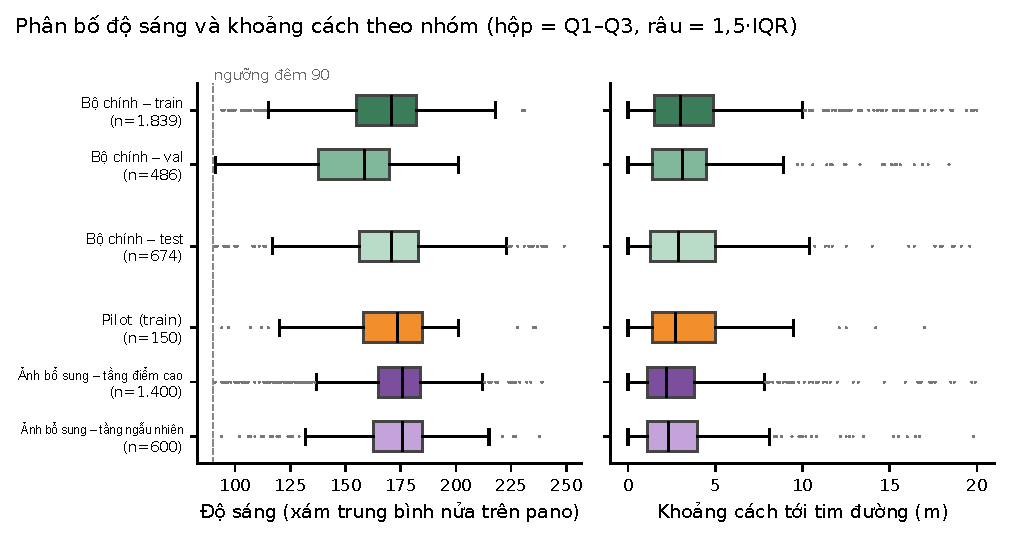
\includegraphics[width=0.95\textwidth]{tab_fig4_brightness_dist_boxplots.pdf}
\caption{Phân bố độ sáng ảnh $360^\circ$ và khoảng cách tới tim đường theo nhóm}
\label{fig:desc}
\end{figure}

\begin{table}[H]
\centering
\caption{Thống kê mô tả các biến số còn lại của metadata}
\label{tab:desc2}
\footnotesize\setlength{\tabcolsep}{3pt}
\begin{tabularx}{\textwidth}{>{\raggedright\arraybackslash}p{0.17\linewidth} r R R R R R R}
\toprule
\textbf{Nhóm} & \textbf{n} & \textbf{Trung bình} & \textbf{Trung vị} & \textbf{Phương sai} & \textbf{Nhỏ nhất} & \textbf{Lớn nhất} & \textbf{IQR} \\
\midrule
\multicolumn{8}{l}{\emph{Vĩ độ ($^\circ$ Bắc)}} \\
Bộ chính, gộp & 2.999 & 10,7751 & 10,7757 & $2{,}7\cdot10^{-4}$ & 10,7501 & 10,8149 & 0,0274 \\
Ảnh bổ sung, gộp & 2.000 & 10,7812 & 10,7860 & $4{,}3\cdot10^{-4}$ & 10,7450 & 10,8150 & 0,0359 \\
\multicolumn{8}{l}{\emph{Kinh độ ($^\circ$ Đông)}} \\
Bộ chính, gộp & 2.999 & 106,6792 & 106,6813 & $2{,}3\cdot10^{-4}$ & 106,6500 & 106,7059 & 0,0285 \\
Ảnh bổ sung, gộp & 2.000 & 106,6813 & 106,6813 & $3{,}1\cdot10^{-4}$ & 106,6500 & 106,7234 & 0,0291 \\
\multicolumn{8}{l}{\emph{Hướng di chuyển của xe ($^\circ$, 0 = hướng Bắc)}} \\
Bộ chính, gộp & 2.999 & 166,5 & 164,7 & 10.589,6 & 0,0 & 360,0 & 193,3 \\
Ảnh bổ sung, gộp & 2.000 & 178,0 & 167,5 & 10.050,7 & 0,1 & 359,6 & 180,3 \\
\multicolumn{8}{l}{\emph{Điểm của bộ chọn ảnh (chỉ có ở ảnh bổ sung, thang 0--1)}} \\
Tầng điểm cao & 1.400 & 0,799 & 0,798 & 0,012 & 0,610 & 0,996 & 0,191 \\
Tầng ngẫu nhiên & 600 & 0,231 & 0,188 & 0,032 & 0,001 & 0,607 & 0,286 \\
\multicolumn{8}{l}{\emph{Thời gian gán một ảnh (giây, tính theo lượt gán)}} \\
Bộ chính & 4.435 & 51,5 & 3,7 & 2.285.741 & 0,5 & 77.451 & 6,9 \\
Ảnh bổ sung & 2.000 & 13,9 & 4,5 & 24.475 & 0,9 & 6.678 & 5,3 \\
\bottomrule
\end{tabularx}
\note{Góc cắt không được đưa vào bảng vì là hằng số ($60^\circ$ về bên phải) với mọi ảnh.}
\end{table}

\begin{itemize}
  \item \textbf{Độ sáng} (bảng~\ref{tab:desc}, hình~\ref{fig:desc}). Không ảnh nào có độ sáng dưới ngưỡng lọc ảnh đêm (nhỏ nhất là 91). Ảnh tập val tối hơn các nhóm khác (trung vị 158,5 so với 171); do val chỉ có 3 đường, đây có thể là đặc điểm riêng của ba đường này.
  \item \textbf{Khoảng cách tới tim đường} bị giới hạn trên ở 20 m theo quy tắc gắn đường. Ảnh bổ sung gần tim đường hơn (trung vị 2,2 m so với 3,0 m), phù hợp với việc 71\% ảnh bổ sung đến từ đường nhỏ.
  \item \textbf{Tọa độ} (bảng~\ref{tab:desc2}) nằm trong khung nghiên cứu, trừ 2 ảnh bổ sung lệch ra ngoài dưới 4 m (mục~\ref{sec:eda-quality}). Ảnh bổ sung phân tán rộng hơn bộ chính (IQR của vĩ độ là 0,0359 so với 0,0274) vì đến từ 75 đường thay vì 17 đường.
  \item \textbf{Hướng di chuyển của xe} trải đều trên toàn dải 0--$360^\circ$ (IQR xấp xỉ $190^\circ$), không tập trung vào một hướng. Thuộc tính này chỉ được dùng để gắn ảnh vào đường và để cắt ảnh về phía bên phải xe.
  \item \textbf{Điểm của bộ chọn ảnh} (chỉ có ở ảnh bổ sung): tầng điểm cao có trung vị 0,80 (0,61--1,00), tầng ngẫu nhiên có trung vị 0,19 (0,00--0,61).
  \item \textbf{Thời gian gán một ảnh} lệch phải rất mạnh: trung vị là 3,7 giây (bộ chính, 4.435 lượt) và 4,5 giây (ảnh bổ sung), trong khi giá trị lớn nhất lên tới 77.451 giây do một số tác vụ bị để mở. Vì vậy, trung vị là thước đo phù hợp hơn trung bình. Thời gian gán của pilot \textbf{chưa được đo} trong báo cáo này.
\end{itemize}

\subsubsection*{Phân bố theo thuộc tính phân loại}

Hình~\ref{fig:year} và bảng~\ref{tab:month} trình bày phân bố ảnh theo tài khoản chụp, năm chụp và tháng chụp.

\begin{figure}[H]
\centering
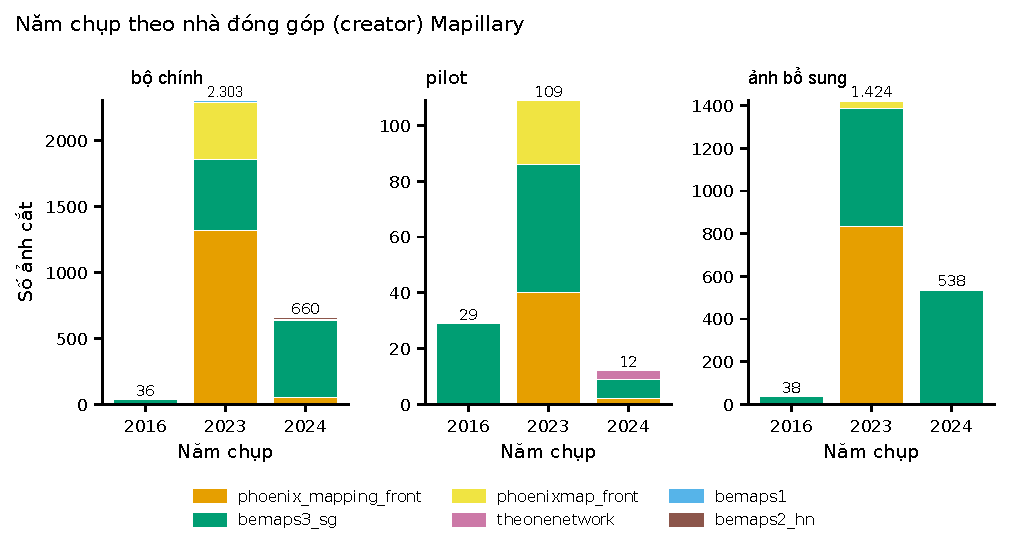
\includegraphics[width=0.95\textwidth]{tab_fig5_year_creator.pdf}
\caption{Số ảnh theo năm chụp và tài khoản chụp}
\label{fig:year}
\end{figure}

\begin{table}[H]
\centering
\caption{Số ảnh theo tháng chụp (theo dấu thời gian của Mapillary)}
\label{tab:month}
\setlength{\tabcolsep}{3.5pt}
\begin{tabular}{l rrrrrrrrrrrr r}
\toprule
\textbf{Tháng} & 1 & 2 & 3 & 4 & 5 & 6 & 7 & 8 & 9 & 10 & 11 & 12 & \textbf{Tổng} \\
\midrule
Bộ chính & 299 & 114 & 0 & 552 & 677 & 234 & 0 & 244 & 54 & 321 & 303 & 201 & 2.999 \\
Ảnh bổ sung & 146 & 204 & 53 & 93 & 461 & 286 & 0 & 55 & 87 & 96 & 342 & 177 & 2.000 \\
\bottomrule
\end{tabular}
\end{table}

\begin{itemize}
  \item \textbf{Tài khoản chụp} (hình~\ref{fig:year}). Hai tài khoản \lab{bemaps3\_sg} và \lab{phoenix\_mapping\_front} chiếm 84\% bộ chính (1.153 và 1.370 trên 2.999 ảnh) và 98\% ảnh bổ sung. Do đó, dữ liệu đến từ rất ít loại thiết bị và cách gắn camera.
  \item \textbf{Năm chụp.} Ở bộ chính, năm 2023 có 2.303 ảnh, năm 2024 có 660 ảnh và năm 2016 có 36 ảnh. Toàn bộ 103 ảnh ghi năm 2016 (trên cả ba phần dữ liệu) đều thuộc tài khoản \lab{bemaps3\_sg} và cùng ghi ngày 01/01/2016; nhiều khả năng đây là ngày mặc định, nên năm 2016 \textbf{không đáng tin cậy}.
  \item \textbf{Tháng chụp} (bảng~\ref{tab:month}). Ảnh được chụp trong 10 tháng khác nhau (bộ chính) và 11 tháng khác nhau (ảnh bổ sung), không có ảnh nào vào tháng 7; ảnh bộ chính tập trung vào tháng 4--5 (41\%). Tháng 1 bao gồm cả các ảnh mang ngày mặc định 01/01/2016.
  \item \textbf{Giờ chụp} trải khắp các khung giờ trong ngày nhưng không đáng tin cậy: ở bộ chính, 1.080/2.999 ảnh (36\%) ghi giờ từ 18 giờ tới trước 6 giờ sáng (ở ảnh bổ sung là 762/2.000, tức 38\%), trong khi mọi ảnh được giữ lại đều vượt ngưỡng độ sáng của bộ lọc ảnh đêm. Vì vậy, giờ chụp không được dùng để lọc ảnh (mục~\ref{sec:cleaning}).
  \item \textbf{Số ảnh mỗi đường.} Bộ chính có 17 đường, mỗi đường 86--348 ảnh (trung vị 150); ảnh bổ sung có 75 đường, mỗi đường 6--157 ảnh (trung vị 21). Hai đường ven kênh Hoàng Sa và Trường Sa\#0 đóng góp 274 ảnh bổ sung (14\%). Hai đường này từng bị loại khỏi bộ chính vì vỉa hè chủ yếu nằm ở một phía và có ít người đi bộ (bước 4, bảng~\ref{tab:steps}). Tuy nhiên, đợt bổ sung chỉ xếp hạng đường theo điểm của bộ chọn ảnh và không áp dụng lại tiêu chí này: hai đường đứng hạng 49 và 56 trong 75 đường, và do có chiều dài lớn nên đóng góp nhiều ảnh. Hai đường này chỉ thuộc train nên không ảnh hưởng tới val/test, nhưng làm tăng tỉ lệ cảnh ven kênh trong train.
\end{itemize}

% ------------------------------------------------------------------------------
\subsection{Phân tích phân bố nhãn}
\label{sec:eda-labels}

Mục này xét mức mất cân bằng giữa các lớp, tỉ lệ từng lớp theo nhóm, thành phần nhãn của tập train sau khi bổ sung, và sự khác biệt theo đường, theo loại vật cản và theo người gán.

\begin{figure}[H]
\centering
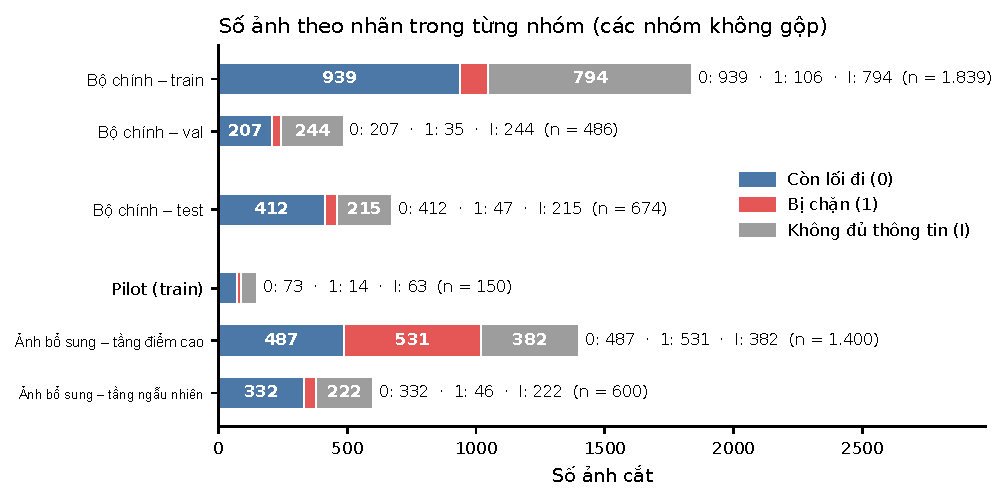
\includegraphics[width=0.95\textwidth]{tab_fig1_label_counts_by_group.pdf}
\caption{Số ảnh theo nhãn trong từng nhóm}
\label{fig:labels}
\end{figure}

\begin{table}[H]
\centering
\caption{Tỉ lệ \lab{Bị chặn} và \lab{Không đủ thông tin} theo nhóm, khoảng tin cậy 95\%}
\label{tab:labels}
\begin{tabularx}{\textwidth}{>{\raggedright\arraybackslash}p{0.2\linewidth} r >{\raggedright\arraybackslash}p{0.2\linewidth} >{\raggedright\arraybackslash}p{0.14\linewidth} r r}
\toprule
\textbf{Nhóm} & \textbf{Ảnh} & \textbf{Bị chặn / hợp lệ [Wilson]} & \textbf{Bootstrap theo đường} & \textbf{Tỉ lệ I} & \textbf{0 : 1} \\
\midrule
Bộ chính, train & 1.839 & 106/1.045 = 10,1\% [8,5; 12,1] & [7,9; 14,1] & 43,2\% & 8,9 \\
Bộ chính, val & 486 & 35/242 = 14,5\% [10,6; 19,4] & [8,2; 19,2] & 50,2\% & 5,9 \\
Bộ chính, test & 674 & 47/459 = 10,2\% [7,8; 13,4] & [5,7; 18,7] & 31,9\% & 8,8 \\
\emph{Bộ chính, gộp} & 2.999 & 188/1.746 = 10,8\% [9,4; 12,3] & [8,7; 13,9] & 41,8\% & 8,3 \\
\midrule
Pilot & 150 & 14/87 = 16,1\% [9,8; 25,2] & [10,0; 18,4] & 42,0\% & 5,2 \\
Ảnh bổ sung, tầng điểm cao & 1.400 & 531/1.018 = 52,2\% [49,1; 55,2] & [47,8; 56,6] & 27,3\% & 0,9 \\
Ảnh bổ sung, tầng ngẫu nhiên & 600 & 46/378 = 12,2\% [9,2; 15,9] & [8,9; 15,3] & 37,0\% & 7,2 \\
\bottomrule
\end{tabularx}
\note{Ảnh hợp lệ là ảnh có nhãn 0 hoặc 1. Bootstrap theo đường: 1.000 lần lấy mẫu lại.}
\end{table}

\begin{itemize}
  \item \textbf{Dữ liệu tự nhiên mất cân bằng mạnh} (hình~\ref{fig:labels}, bảng~\ref{tab:labels}): trong các ảnh hợp lệ của bộ chính, \lab{Còn lối đi} chiếm 89,2\% và \lab{Bị chặn} chiếm 10,8\%, tức cứ khoảng 8 ảnh \lab{Còn lối đi} mới có 1 ảnh \lab{Bị chặn}. Tính trên mọi ảnh, kể cả ảnh \lab{I}, tỉ lệ \lab{Bị chặn} là 6,3\% $[5{,}5;\,7{,}2]$.
  \item \textbf{Tỉ lệ ba lớp \lab{0} / \lab{1} / \lab{I} trên mọi ảnh:} bộ chính gộp 52,0 / 6,3 / 41,8\%; train 51,1 / 5,8 / 43,2\%; val 42,6 / 7,2 / 50,2\%; test 61,1 / 7,0 / 31,9\%; pilot 48,7 / 9,3 / 42,0\%; tầng điểm cao 34,8 / 37,9 / 27,3\%; tầng ngẫu nhiên 55,3 / 7,7 / 37,0\%. Trên toàn bộ dữ liệu: 47,6 / 15,1 / 37,3\%.
  \item \textbf{Khoảng tin cậy của tỉ lệ \lab{Bị chặn} ở ba tập chồng lên nhau} (tỉ lệ lần lượt là 10,1\%, 14,5\% và 10,2\%). Tuy nhiên, điều này chưa đủ để kết luận các tỉ lệ là tương đương.
  \item \textbf{Test chỉ có 47 mẫu dương, val có 35 mẫu dương.} Độ rộng khoảng bootstrap theo đường của test gấp xấp xỉ 2,3 lần độ rộng khoảng Wilson ($[5{,}7;\,18{,}7]$ so với $[7{,}8;\,13{,}4]$, tức 13,0 so với 5,6 điểm phần trăm), nên kết quả đánh giá mô hình trên test sẽ có sai số lớn.
  \item \textbf{Ảnh \lab{I} chiếm 32--50\%} tùy tập. Đây là hạn chế cố hữu của nguồn ảnh chụp từ xe.
  \item \textbf{Tỉ lệ ở pilot và tầng điểm cao không phản ánh phân phối tự nhiên:} tỉ lệ \lab{Bị chặn} của hai nhóm này (16,1\% và 52,2\%) là kết quả của cách lấy mẫu, không phải tỉ lệ thực tế ngoài đường.
  \item \textbf{Tầng ngẫu nhiên của ảnh bổ sung (12,2\%)} có tỉ lệ gần với bộ chính dù được lấy từ các đường khác; hai khoảng tin cậy chồng lên nhau.
\end{itemize}

\begin{figure}[H]
\centering
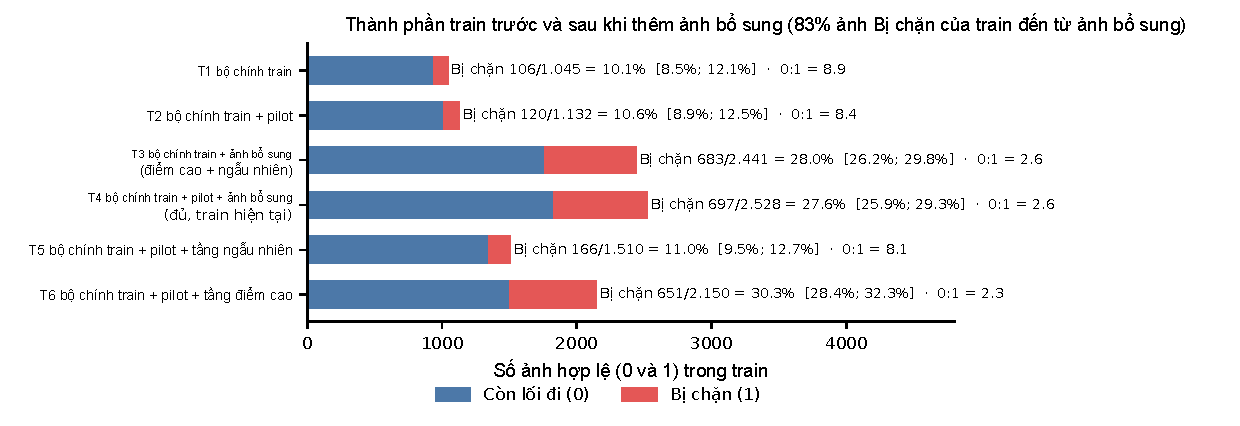
\includegraphics[width=\textwidth]{tab_fig10_train_composition.pdf}
\caption{Thành phần tập train trước và sau khi thêm pilot và ảnh bổ sung (chỉ tính ảnh hợp lệ)}
\label{fig:train}
\end{figure}

\textbf{Tập train sau khi bổ sung} (hình~\ref{fig:train}). Train hiện có 2.528 ảnh hợp lệ, trong đó 697 mẫu dương (27,6\%, tỉ lệ 0:1 là 2,6), so với 1.132 ảnh hợp lệ và 120 mẫu dương (10,6\%) trước khi bổ sung. 577 trong 697 mẫu dương (83\%) đến từ ảnh bổ sung. Hệ quả là phân phối nhãn của train khác với val/test (27,6\% so với khoảng 10--15\%); khi huấn luyện cần tính tới độ lệch này, đồng thời nên báo cáo thêm kết quả khi chỉ huấn luyện trên phần dữ liệu tự nhiên.

\begin{figure}[H]
\centering
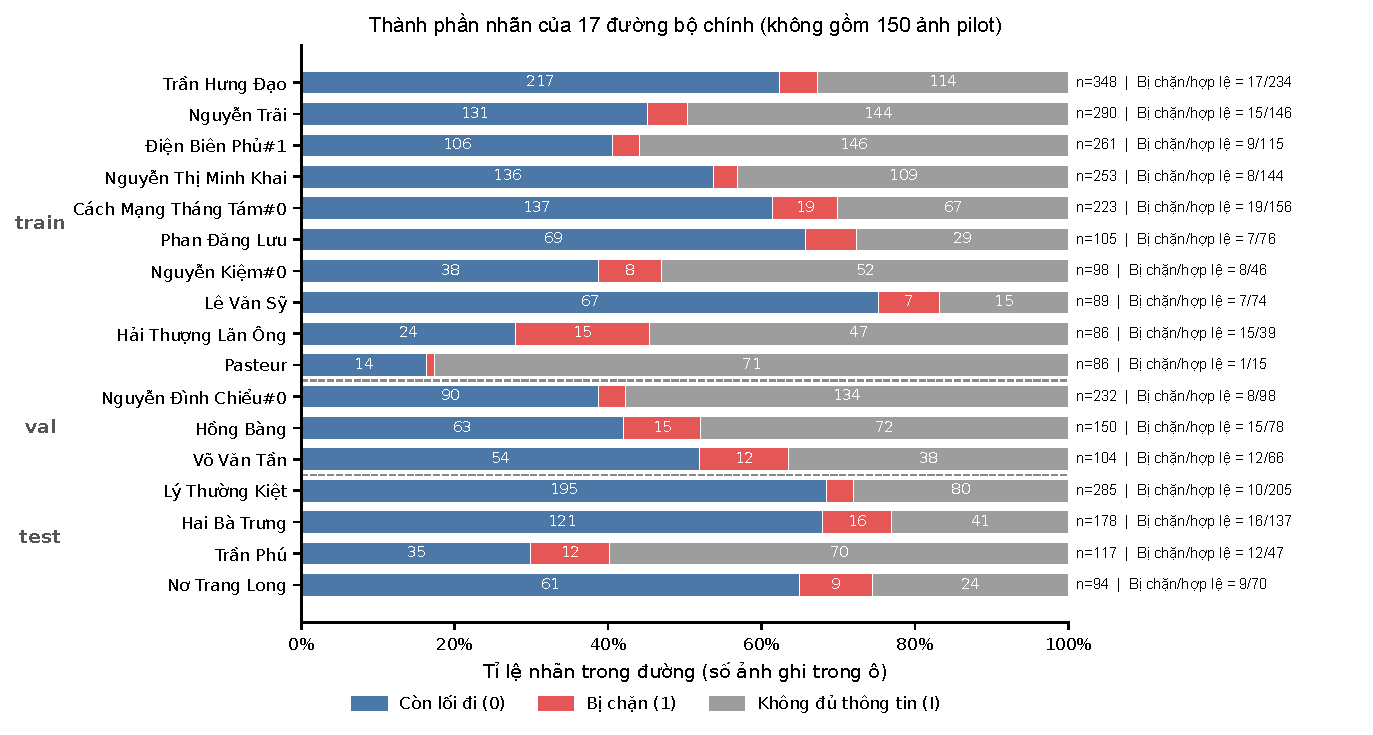
\includegraphics[width=\textwidth]{tab_fig3a_main_street_composition.pdf}
\caption{Thành phần nhãn của 17 đường thuộc bộ chính (không gồm pilot)}
\label{fig:streets}
\end{figure}

\textbf{Theo đường} (hình~\ref{fig:streets}). Tỉ lệ nhãn khác nhau đáng kể giữa các đường: tỉ lệ \lab{Bị chặn} trên ảnh hợp lệ dao động từ 4,9\% (Lý Thường Kiệt, 10/205) tới 38,5\% (Hải Thượng Lãn Ông, 15/39); tỉ lệ \lab{I} dao động từ 17\% (Lê Văn Sỹ) tới 83\% (Pasteur, đường một chiều). Ở ảnh bổ sung, trong 25 đường có ít nhất 20 ảnh hợp lệ, tỉ lệ \lab{Bị chặn} dao động từ 11,1\% (Bạch Đằng\#0, 4/36) tới 76,2\% (Ung Văn Khiêm, 16/21), trung vị 40,0\%; các tỉ lệ này gộp hai tầng nên chịu ảnh hưởng của cách chọn ảnh. Tuyến đường là thuộc tính có mức liên hệ với nhãn mạnh nhất (mục~\ref{sec:eda-rel}), vì vậy việc chia tập theo đường là cần thiết để tránh đánh giá quá lạc quan.

\begin{figure}[H]
\centering
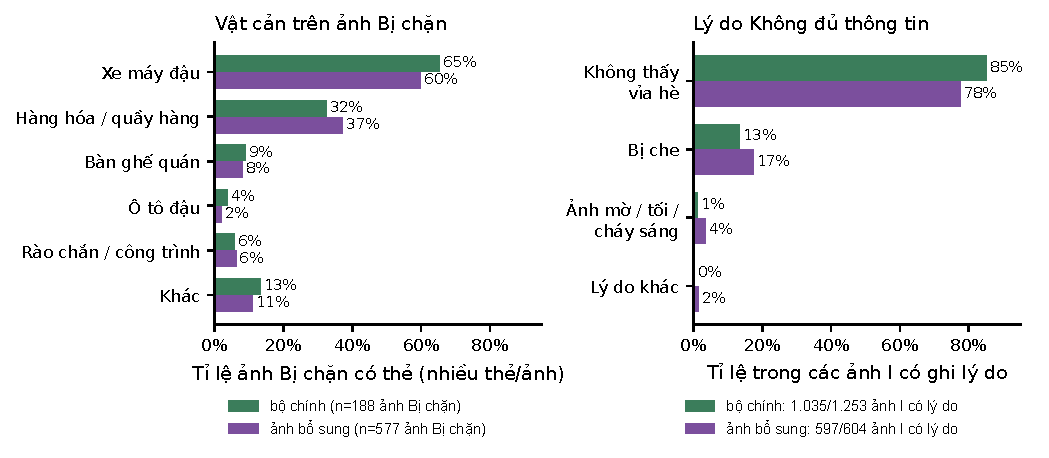
\includegraphics[width=0.95\textwidth]{tab_fig7_obstacles_reasons.pdf}
\caption{Loại vật cản trên ảnh \lab{Bị chặn} và lý do gán nhãn \lab{Không đủ thông tin}, bộ chính so với ảnh bổ sung}
\label{fig:obstacles}
\end{figure}

\textbf{Đa dạng của vật cản và lý do gán nhãn \lab{I}} (hình~\ref{fig:obstacles}).
\begin{itemize}
  \item Trên ảnh \lab{Bị chặn}, xe máy đậu là loại vật cản phổ biến nhất (bộ chính 123/188 ảnh, 65\%; ảnh bổ sung 346/577 ảnh, 60\%), tiếp theo là hàng hóa và quầy hàng (32\% và 37\%). Ô tô đậu hiếm gặp (4\% và 2\%). Một ảnh có thể có nhiều loại vật cản. Cơ cấu vật cản của hai phần dữ liệu khá tương đồng.
  \item Lý do gán \lab{I} chủ yếu là không thấy vỉa hè (bộ chính 880/1.035 ảnh có ghi lý do, 85\%; ảnh bổ sung 463/597 ảnh, 78\%), tiếp theo là vỉa hè bị che khuất. Ảnh mờ, tối hoặc cháy sáng chỉ có 12 và 21 ảnh.
  \item Thẻ vật cản là thông tin phụ, không bắt buộc: 13 ảnh \lab{Bị chặn} của bộ chính và 6 ảnh bổ sung không có thẻ nào. Thẻ vật cản của pilot \textbf{chưa được thống kê}.
\end{itemize}
\note{Thẻ vật cản của một ảnh là hợp của các thẻ từ những lượt gán nhãn 1 cho ảnh đó.}

\begin{figure}[H]
\centering
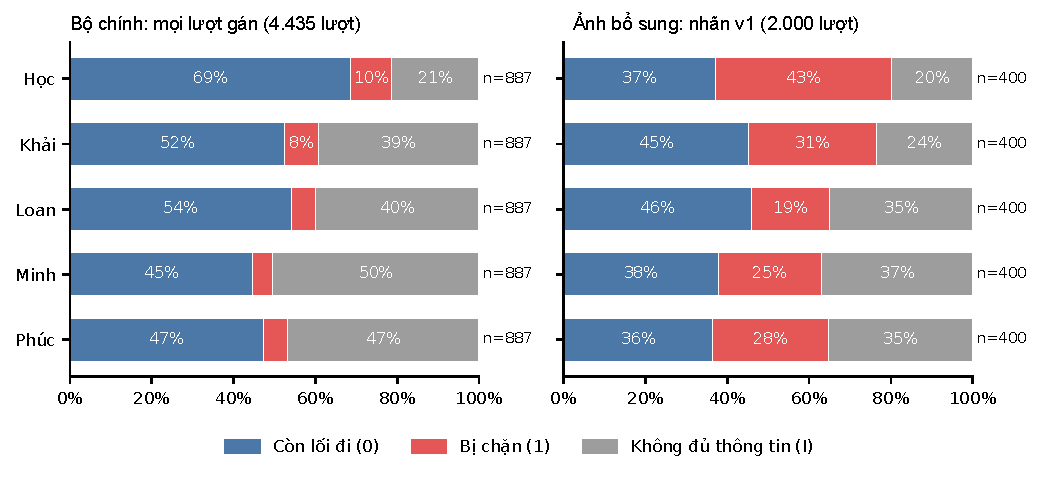
\includegraphics[width=0.95\textwidth]{tab_fig8_annotator_label_shares.pdf}
\caption{Tỉ lệ nhãn theo người gán; phần ảnh bổ sung dùng nhãn của từng người trước kiểm tra chéo}
\label{fig:annotators}
\end{figure}

\textbf{Theo người gán} (hình~\ref{fig:annotators}). Ở ảnh bổ sung, ảnh được chia ngẫu nhiên cho người gán nên chênh lệch giữa người gán gợi ý sự khác biệt trong cách gán, nhưng cần cho nhiều người cùng gán một mẫu ảnh để xác nhận: tỉ lệ \lab{Bị chặn} dao động từ 19\% (Loan) tới 43\% (Học). Ở bộ chính, mỗi người gán một phần ảnh khác nhau (hai người gán test, hai người gán val), nên tỉ lệ theo người gán bị lẫn với ảnh hưởng của tập và không so sánh trực tiếp được.

% ------------------------------------------------------------------------------
\subsection{Phân tích mối quan hệ giữa các thuộc tính}
\label{sec:eda-rel}

Đầu vào của mô hình là ảnh, không phải metadata. Mục này trả lời hai câu hỏi: các thuộc tính metadata có trùng lặp thông tin với nhau không, và có thuộc tính nào liên hệ với nhãn tới mức cần đề phòng mô hình học lối tắt (shortcut learning) không. Với biến số, mức liên hệ với nhãn được đo bằng AUC (diện tích dưới đường cong ROC; 0,5 nghĩa là không phân biệt được hai lớp); với biến phân loại, mức liên hệ được đo bằng Cramér's V hiệu chỉnh độ chệch.

\begin{figure}[H]
\centering
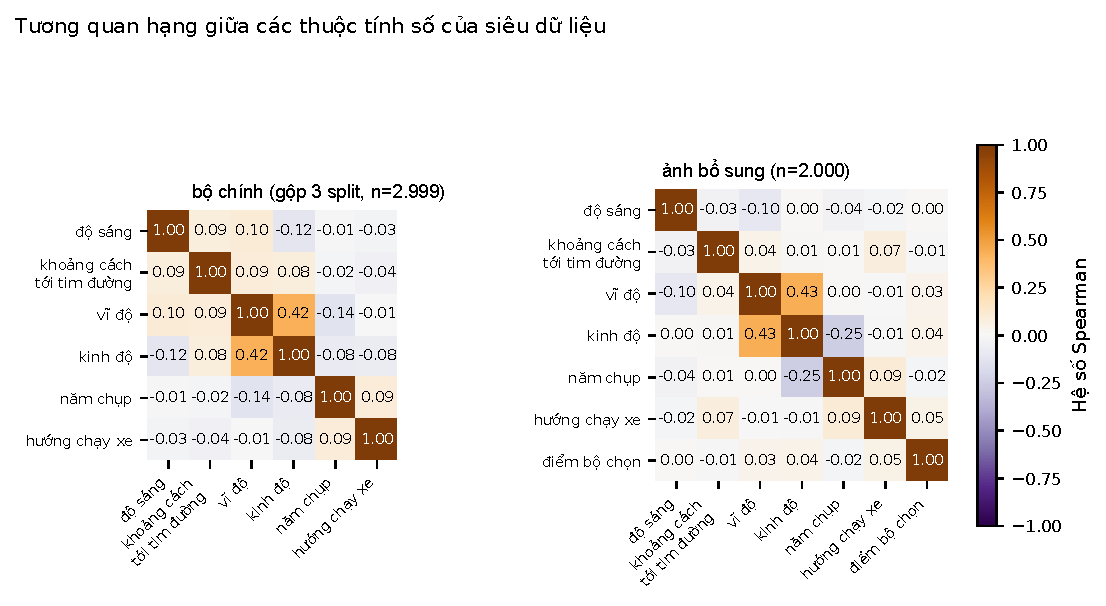
\includegraphics[width=0.95\textwidth]{tab_fig6_spearman_heatmap.pdf}
\caption{Tương quan hạng Spearman giữa các thuộc tính số của metadata}
\label{fig:spearman}
\end{figure}

\begin{itemize}
  \item \textbf{Tương quan} (hình~\ref{fig:spearman}). Cặp duy nhất có tương quan đáng kể là vĩ độ--kinh độ ($\rho = 0{,}42$ ở bộ chính, 0,43 ở ảnh bổ sung), do hình dạng khu vực nghiên cứu và hướng của các tuyến đường. Mọi cặp còn lại có $|\rho| \le 0{,}14$ ở bộ chính và $\le 0{,}25$ ở ảnh bổ sung.
  \item \textbf{Đa cộng tuyến.} Hệ số phóng đại phương sai (VIF) lớn nhất là 1,27 (vĩ độ) và 1,25 (kinh độ) ở bộ chính, do hai biến này tương quan với nhau; các biến khác đều dưới 1,1. Không thấy dấu hiệu đa cộng tuyến đáng kể giữa các biến được kiểm tra.
\end{itemize}

\begin{table}[H]
\centering
\caption{Liên hệ giữa thuộc tính và nhãn \lab{Bị chặn} so với \lab{Còn lối đi} (ảnh hợp lệ)}
\label{tab:assoc}
\begin{tabularx}{\textwidth}{>{\raggedright\arraybackslash}p{0.3\linewidth} L L}
\toprule
\textbf{Thuộc tính} & \textbf{Bộ chính, gộp (n = 1.746)} & \textbf{Ảnh bổ sung (n = 1.396)} \\
\midrule
\multicolumn{3}{l}{\emph{Biến số: AUC (0,5 = không phân biệt), khoảng bootstrap theo đường}} \\
Độ sáng ảnh $360^\circ$ & 0,53 [0,47; 0,59] & 0,49 [0,45; 0,53] \\
Khoảng cách tới tim đường & 0,54 [0,50; 0,58] & 0,46 [0,43; 0,49] \\
Vĩ độ & 0,45 [0,37; 0,52] & khoảng tin cậy chứa 0,5 \\
Kinh độ & 0,45 [0,35; 0,54] & khoảng tin cậy chứa 0,5 \\
Điểm của bộ chọn ảnh & không có & 0,78 [0,75; 0,81] \\
\midrule
\multicolumn{3}{l}{\emph{Biến phân loại: Cramér's V hiệu chỉnh độ chệch~\cite{bergsma2013cramer} (0 = không liên hệ)}} \\
Tuyến đường & 0,18 & 0,29 \\
Loại đường & 0,00 (chỉ 2 mức) & 0,14 [0,06; 0,24] \\
Tài khoản chụp & 0,00 & 0,03 \\
Năm chụp & 0,02 & 0,03 \\
\bottomrule
\end{tabularx}
\note{Giá trị $p$ của các kiểm định này được tính với giả định ảnh độc lập nên quá lạc quan; báo cáo chỉ dựa vào độ lớn hiệu ứng.}
\end{table}

\begin{itemize}
  \item \textbf{Tuyến đường là thuộc tính có mức liên hệ với nhãn mạnh nhất}, với cả \lab{Bị chặn} (V = 0,18) lẫn \lab{I} (V = 0,28 ở bộ chính). Đây là lý do chính để chia tập theo đường.
  \item \textbf{Loại đường} (theo phân loại của OSM) có liên hệ với nhãn ở ảnh bổ sung: trong tầng ngẫu nhiên, tỉ lệ \lab{Bị chặn} trên ảnh hợp lệ là 13,7\% ở đường nhánh (tertiary, 34/248) và 20\% ở đường khu dân cư (residential, 4/20), so với 7,0\% ở đường chính (primary, 3/43) và 7,5\% ở đường cấp hai (secondary, 5/67). Do cỡ mẫu các nhóm nhỏ, khoảng tin cậy rộng. Bộ chính chỉ gồm đường lớn nên không kiểm tra được.
  \item \textbf{Độ sáng, khoảng cách, tọa độ, tài khoản chụp và năm chụp} gần như không phân biệt được nhãn: mọi khoảng tin cậy của bộ chính đều chứa 0,5.
  \item \textbf{Điểm của bộ chọn ảnh} liên hệ mạnh với nhãn ở ảnh bổ sung (AUC 0,78). Đây là hệ quả của cách chọn ảnh, và cũng là lý do điểm này không được dùng làm đặc trưng hay nhãn.
\end{itemize}

Riêng trong train của bộ chính, kinh độ có AUC 0,37 $[0{,}28;\,0{,}47]$: ảnh \lab{Bị chặn} lệch về phía tây. Vì train chỉ có 10 đường, đây nhiều khả năng là khác biệt giữa các đường, không phải một quy luật địa lý.

% ------------------------------------------------------------------------------
\subsection{Kiểm tra chất lượng dữ liệu}
\label{sec:eda-quality}

Mục này trình bày các kiểm tra về tính hợp lệ, ngoại lệ, trùng lặp và rò rỉ giữa các tập. Trong mục này, \emph{kiểm tra trực quan} là quan sát trên các bảng ảnh tổng hợp (contact sheet), không phải phép đo.

\subsubsection*{Tính hợp lệ và nhất quán}

Script EDA dạng bảng thực hiện 71 phép kiểm tra tự động: 62 phép đạt và 9 phép không đạt (bảng~\ref{tab:checks}). Không có dữ liệu nào bị chỉnh sửa trong quá trình kiểm tra.

\begin{table}[H]
\centering
\caption{Kết quả kiểm tra tính hợp lệ và nhất quán}
\label{tab:checks}
\begin{tabularx}{\textwidth}{>{\raggedright\arraybackslash}p{0.37\linewidth} c L}
\toprule
\textbf{Kiểm tra} & \textbf{Kết quả} & \textbf{Chi tiết và cách xử lý} \\
\midrule
Mã ảnh là duy nhất trong và giữa ba bảng nhãn & Đạt & 5.149 mã khác nhau \\
Nhãn khớp 1:1 với manifest & Đạt & Cả ba phần dữ liệu \\
Tập và đường khớp giữa nhãn, manifest và cấu hình & Đạt & \\
Không đường nào thuộc hai tập; không vị trí 25 m nào thuộc hai tập & Đạt & Ảnh bổ sung không dùng chung đường với bộ chính \\
Không ảnh $360^\circ$ nào được dùng hai lần & Đạt & Trong từng phần và giữa ba phần \\
Nhãn thuộc \{0, 1, I\}; cắt phía phải; góc $60^\circ$; giấy phép hợp lệ & Đạt & \\
Mọi ảnh được giữ lại có độ sáng trên ngưỡng lọc ảnh đêm & Đạt & Nhỏ nhất là 91; ảnh bị loại có độ sáng 27--90. Phép kiểm tra chặt ``mọi ảnh bị loại đều dưới 90'' không đạt vì 1 ảnh trong kho ứng viên bổ sung ghi đúng 90 (giá trị đã làm tròn) \\
\midrule
Ảnh \lab{I} có ghi lý do & Không đạt & 281 + 7 ảnh, thiếu do cấu trúc quy trình (mục~\ref{sec:eda-desc}). Giữ nguyên \\
Thẻ vật cản chỉ xuất hiện khi lượt gán chọn \lab{1} & Không đạt & 285/4.435 lượt (bộ chính) và 119/2.000 lượt (ảnh bổ sung) có thẻ nhưng nhãn là 0 hoặc I. Thống kê vật cản chỉ dùng các lượt chọn \lab{1} \\
Tọa độ nằm trong khung nghiên cứu & Không đạt & 2 ảnh bổ sung nằm ngoài khung dưới 4 m (do làm tròn biên khung). Giữ nguyên \\
Hướng di chuyển nằm trong $[0, 360)$ & Không đạt & 1 ảnh ghi 360,0 (tương đương 0). Không ảnh hưởng tới phân tích \\
Ngày chụp không phải ngày mặc định & Không đạt & 103 ảnh ghi ngày 01/01/2016. Năm chụp không được dùng để lọc hay chia tập \\
Ảnh pilot không trùng vị trí với ảnh bộ chính & Không đạt & 5 ảnh pilot cách ảnh bộ chính dưới 5 m (gần nhất 2,9 m). Cả hai phía đều thuộc train nên không gây rò rỉ giữa các tập \\
\bottomrule
\end{tabularx}
\end{table}

\subsubsection*{Ngoại lệ và dữ liệu bất thường}

\begin{itemize}
  \item \textbf{Metadata.} Theo quy tắc $1{,}5\times$IQR~\cite{tukey1977eda}, bộ chính có 81 ảnh ngoại lệ về độ sáng ảnh $360^\circ$ (63 thấp, 18 cao) và 113 ảnh có khoảng cách tới tim đường lớn; ở ảnh bổ sung, các con số tương ứng là 113 và 71 ảnh. Đây là phần đuôi của các phân bố lệch, không phải lỗi nhập liệu; mọi giá trị đều nằm trong miền hợp lệ (độ sáng 91--249, khoảng cách 0--20 m).
  \item \textbf{Ảnh cắt.} Trên 5.149 ảnh có 87 ảnh ngoại lệ về độ sáng (7 ảnh quá tối, 80 ảnh quá sáng), 36 ảnh ngoại lệ về độ tương phản và 115 ảnh có độ nét rất thấp (trên thang log). Tổng cộng 308 ảnh vượt ít nhất một ngưỡng ngoại lệ.
  \item \textbf{Ảnh cháy sáng} (trên 20\% điểm ảnh bão hòa): 128 ảnh. Tỉ lệ ở test (33 ảnh, 4,9\%) và val (25 ảnh, 5,1\%) cao hơn ở train (36 ảnh, 2,0\%); 27/33 ảnh cháy sáng của test thuộc đường Hai Bà Trưng.
  \item \textbf{Kiểm tra trực quan các ảnh ngoại lệ:} ảnh tối nhất phần lớn chụp trong bóng râm, dưới gầm cầu vượt hoặc khi trời âm u, không phải ảnh đêm; ảnh sáng nhất bị phơi sáng quá mức nhưng nhiều ảnh vẫn quan sát được vỉa hè; ảnh mờ nhất phần lớn là cảnh tối hoặc bị nhòe do chuyển động.
  \item \textbf{Cách xử lý:} không loại ảnh ngoại lệ nào. Các ảnh có chất lượng kém tới mức không đánh giá được đã được người gán xếp vào nhãn \lab{I}; phần còn lại phản ánh điều kiện chụp thực tế mà mô hình cần xử lý được.
\end{itemize}

\textbf{Kiểm tra bộ lọc ảnh đêm} (việc còn tồn đọng từ trước). 58 ảnh $360^\circ$ bị loại của bộ chính và 58 ảnh được giữ lại có độ sáng thấp nhất đã được kiểm tra trực quan. Khoảng 48/58 ảnh bị loại đúng là ảnh đêm; 9 ảnh có vẻ được chụp ban ngày dưới tán cây dày và 1 ảnh chụp lúc chạng vạng (độ sáng 68--89). Trong 58 ảnh được giữ lại đã xem, chưa thấy ảnh đêm nào, khoảng 3 ảnh được chụp lúc chạng vạng; kết quả này chưa đủ để khẳng định cho toàn bộ ảnh được giữ lại. Khoảng 10 ảnh bị loại nhầm (9 ảnh ban ngày, 1 ảnh chạng vạng), tương ứng khoảng 0,3\% của 3.057 ảnh đầu vào. 38 ảnh bị loại trong kho ứng viên bổ sung \textbf{chưa được xem lại}.
\note{Các bảng ảnh tổng hợp dùng nội bộ có chứa ảnh val/test nên không được đưa vào báo cáo.}

\subsubsection*{Trùng lặp và gần trùng}

\begin{itemize}
  \item \textbf{Trùng lặp tuyệt đối: không có.} Không có hai file nào trùng mã băm MD5, không có hai ảnh nào trùng điểm ảnh sau khi giải nén, và không ảnh $360^\circ$ nào xuất hiện hai lần (n = 5.149).
  \item \textbf{Bản sao gần như y hệt: không có.} Không có cặp ảnh nào có khoảng cách dHash $\le 4$ (mã băm 64 bit). Cặp gần nhất giữa các tập có dHash bằng 6; kiểm tra trực quan cho thấy đây là hai địa điểm khác nhau có cùng một mảng trời sáng.
  \item \textbf{Cùng vị trí, khác ngày.} Có 1.709 vị trí có hai ảnh chụp ở hai ngày khác nhau (bộ chính 1.363, ảnh bổ sung 346), và hai ảnh của mỗi vị trí luôn thuộc cùng một tập. Theo phép đo, các cặp này \emph{không} giống nhau về nội dung: dHash nhỏ nhất là 12 (trung vị 31, tương đương các cặp ảnh khác đường); độ tương đồng cosine giữa các vector đặc trưng DINOv2 có trung vị 0,63 và lớn nhất 0,905. Do hai ngày chụp có xe cộ, hàng quán và ánh sáng khác nhau, việc giữ cả hai ảnh là hợp lý.
  \item \textbf{Hệ quả về phương pháp:} cả dHash lẫn độ tương đồng cosine đều không phân biệt được ``cùng một địa điểm'' với ``cảnh tương tự'' (hình~\ref{fig:dupdist}); chỉ khoảng cách địa lý làm được việc này. Vì vậy, báo cáo không đặt ngưỡng gần trùng dựa trên nội dung ảnh.
\end{itemize}

\begin{figure}[H]
\centering
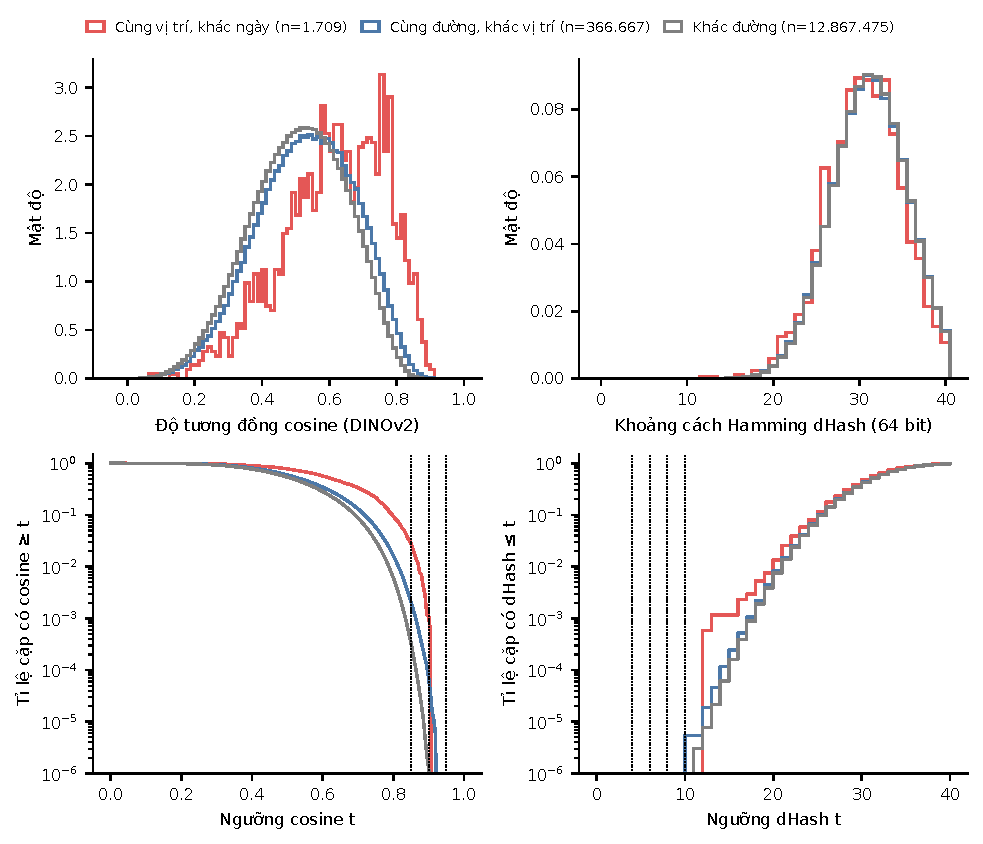
\includegraphics[width=0.92\textwidth]{dup_distance_distributions.pdf}
\caption{Phân bố độ tương đồng giữa các cặp ảnh: cùng vị trí khác ngày, cùng đường khác vị trí, khác đường}
\label{fig:dupdist}
\end{figure}

\subsubsection*{Rò rỉ giữa các tập}

Rò rỉ giữa các tập được đánh giá theo hai cách: theo nội dung ảnh và theo vị trí địa lý (hình~\ref{fig:map}).

\begin{figure}[H]
\centering
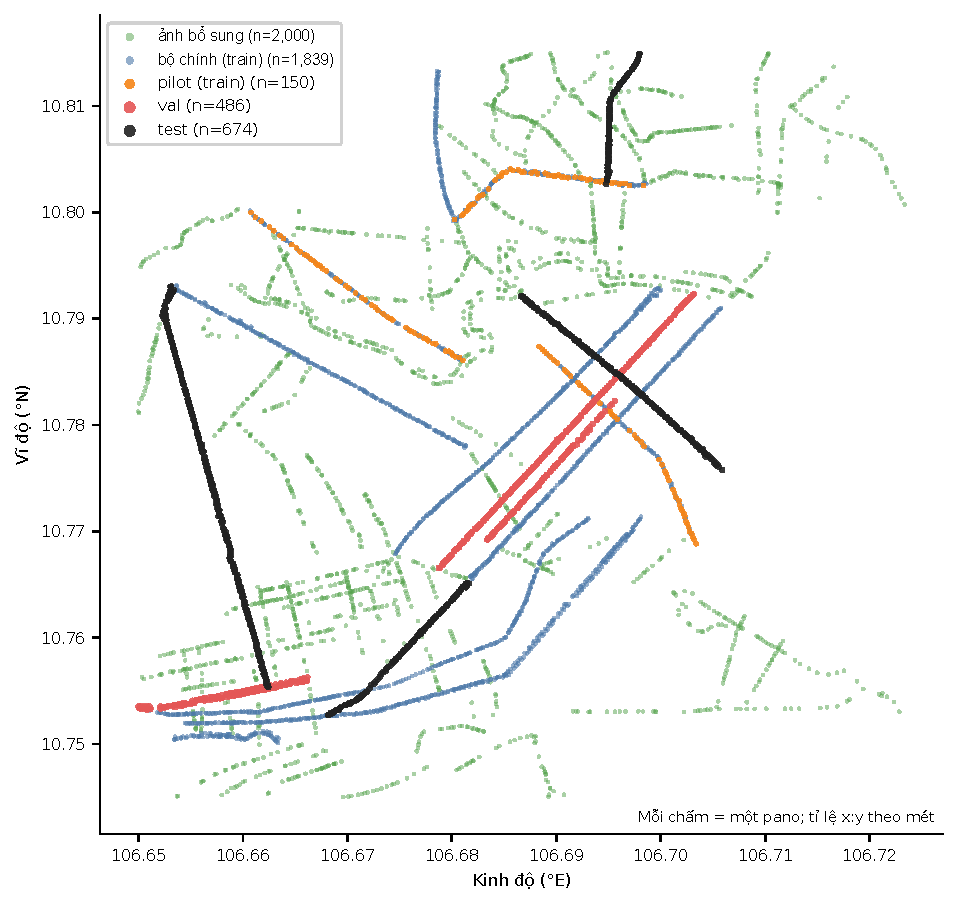
\includegraphics[width=0.8\textwidth]{dup_map_positions.pdf}
\caption{Vị trí của mọi ảnh theo tập. Các đường val/test cắt đường train tại giao lộ}
\label{fig:map}
\end{figure}

\textbf{Theo nội dung ảnh.} Với mỗi ảnh val/test, ảnh giống nhất ở phía train (bộ chính, pilot, ảnh bổ sung) được tìm theo độ tương đồng cosine.
\begin{itemize}
  \item Độ tương đồng với ảnh train gần nhất: val có trung vị 0,78, lớn nhất 0,909; test có trung vị 0,79, lớn nhất 0,904. Phân bố này trùng với mức tham chiếu giữa các đường train với nhau (trung vị 0,81, lớn nhất 0,933); nói cách khác, mức tương đồng giữa val/test và train không cao hơn mức tương đồng giữa hai đường train bất kỳ.
  \item Có 7 ảnh val/test có độ tương đồng cosine $\ge 0{,}90$ với một ảnh train, nhưng cả 7 cặp đều cách nhau 778--3.585 m. Kiểm tra trực quan 20 cặp giống nhau nhất cho thấy đều là hai địa điểm khác nhau có cùng kiểu cảnh (dãy nhà phố, người đi xe máy ở tiền cảnh).
\end{itemize}

\textbf{Theo vị trí địa lý.} Việc chia theo đường không ngăn được trường hợp đường val/test \emph{cắt} đường train tại giao lộ. Bảng~\ref{tab:spatial} thống kê số ảnh val/test nằm gần ảnh phía train.

\begin{table}[H]
\centering
\caption{Số ảnh val/test nằm gần một ảnh phía train}
\label{tab:spatial}
\begin{tabularx}{\textwidth}{>{\raggedright\arraybackslash}p{0.3\linewidth} R R R R R}
\toprule
\textbf{Cặp} & \textbf{Gần nhất (m)} & \textbf{< 15 m} & \textbf{< 25 m} & \textbf{< 40 m} & \textbf{< 100 m} \\
\midrule
Val (486) -- train bộ chính & 1,5 & 6 & 6 & 14 & 47 \\
Val -- pilot & 17,9 & 0 & 1 & 5 & 17 \\
Val -- ảnh bổ sung & 41,6 & 0 & 0 & 0 & 71 \\
Test (674) -- train bộ chính & 7,1 & 8 & 18 & 34 & 88 \\
Test -- pilot & 20,9 & 0 & 2 & 4 & 7 \\
Test -- ảnh bổ sung & 34,3 & 0 & 0 & 3 & 116 \\
\bottomrule
\end{tabularx}
\end{table}

\begin{itemize}
  \item \textbf{52 trên 1.160 ảnh val/test (4,5\%) nằm cách một ảnh train dưới 40 m}, liên quan tới 47 ảnh phía train và 13 cặp đường giao nhau (ví dụ Hồng Bàng -- Nguyễn Trãi, Lý Thường Kiệt -- Cách Mạng Tháng Tám, Hai Bà Trưng -- Điện Biên Phủ).
  \item Kiểm tra trực quan 20 cặp gần nhau nhất (1--14 m): phần lớn nhìn về hai hướng khác nhau, nhưng một số cặp thấy cùng một góc phố (cùng cột điện, biển quảng cáo, hàng rào). Phép đo theo nội dung không phát hiện được các cặp này: độ tương đồng cosine lớn nhất của chúng chỉ là 0,82.
  \item \textbf{Ảnh bổ sung tuân thủ quy tắc 40 m}, trừ 1 ảnh cách ảnh test 34,3 m (do quy tắc được áp dụng cho tâm của ô 25 m, không áp dụng cho từng ảnh).
  \item 53 trên 551 chuỗi ảnh Mapillary chứa ảnh của cả phía train lẫn val/test (cùng một lượt xe chạy qua nhiều đường). Đây không phải rò rỉ nội dung, nhưng cho thấy cùng một thiết bị và điều kiện chụp xuất hiện ở cả hai phía.
\end{itemize}

\textbf{Kế hoạch xử lý} (chưa thực hiện, cần nhóm quyết định trước khi khóa chia tập): loại khỏi train các ảnh cách ảnh val/test dưới 40 m, tương tự quy tắc đã áp dụng cho ảnh bổ sung. Quy tắc này chỉ dùng tọa độ, không dùng nhãn val/test, và loại tối đa 47 ảnh train. Phương án thay thế là giữ nguyên dữ liệu và báo cáo kết quả test kèm một lượt đánh giá loại bỏ 52 ảnh gần giao lộ.

\subsubsection*{Mức khác biệt giữa ảnh bổ sung và bộ chính}

Một bộ phân loại tuyến tính trên vector đặc trưng DINOv2, không dùng nhãn vật cản, được huấn luyện để phân biệt hai nhóm ảnh; AUC bằng 0,5 nghĩa là không phân biệt được. Việc đánh giá dùng xác thực chéo (cross-validation) chia theo đường. Bảng~\ref{tab:domain} trình bày kết quả; hình~\ref{fig:tsne} minh họa phân bố các vector đặc trưng bằng t-SNE.

\begin{figure}[H]
\centering
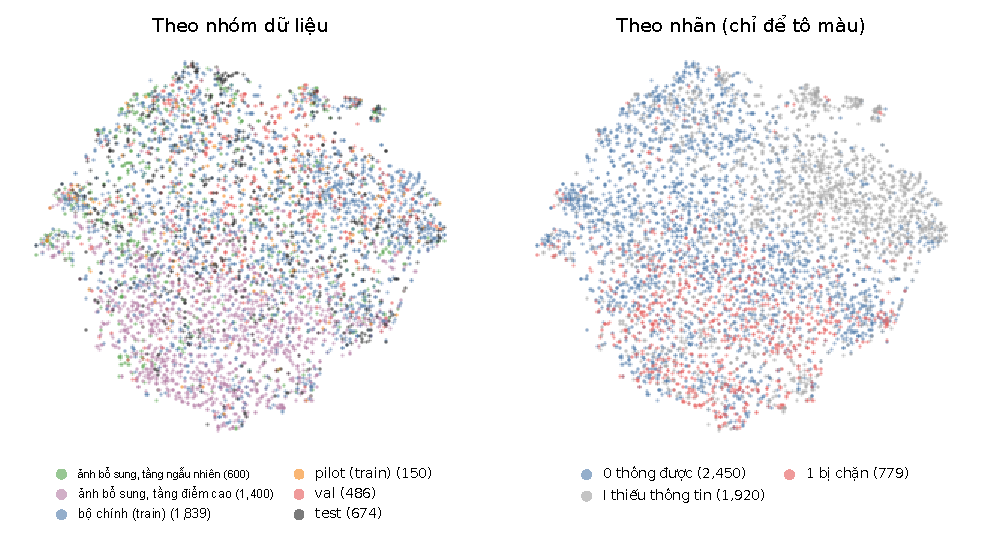
\includegraphics[width=\textwidth]{dup_tsne.pdf}
\caption[Hình chiếu t-SNE của embedding DINOv2 cho 5.149 ảnh, tô theo nhóm và theo nhãn]{Hình chiếu t-SNE~\cite{maaten2008tsne} của embedding DINOv2 cho 5.149 ảnh, tô màu theo nhóm và theo nhãn (nhãn chỉ dùng để tô màu)}
\label{fig:tsne}
\end{figure}

\begin{table}[H]
\centering
\caption{Mức phân biệt được giữa các nhóm ảnh (AUC của bộ phân loại miền)}
\label{tab:domain}
\begin{tabularx}{\textwidth}{>{\raggedright\arraybackslash}p{0.5\linewidth} R L}
\toprule
\textbf{So sánh} & \textbf{AUC} & \textbf{Diễn giải} \\
\midrule
Train bộ chính -- ảnh bổ sung, tầng điểm cao & 0,95 & Khác biệt rõ \\
Train bộ chính -- ảnh bổ sung, tầng ngẫu nhiên & 0,70 & Khác biệt vừa phải \\
Ảnh bổ sung -- val + test & 0,83 & Khác biệt rõ \\
Train bộ chính -- val + test & 0,47 & Không phân biệt được \\
Đối chứng: chia đôi ngẫu nhiên các đường train & 0,51 & Mức nền \\
\bottomrule
\end{tabularx}
\note{Trung bình qua các fold; độ lệch chuẩn giữa các fold 0,02--0,08.}
\end{table}

\begin{itemize}
  \item \textbf{Chưa phát hiện khác biệt miền ảnh giữa train bộ chính và val/test bằng bộ phân loại đã dùng} (AUC gần 0,5); tuy nhiên, kết quả này chưa chứng minh hai phân phối giống nhau. Với chỉ 17 đường, phép đo không đủ nhạy để phát hiện các khác biệt nhỏ.
  \item \textbf{Giá trị gộp 0,47 che khuất các giá trị dao động mạnh khi tách riêng:} train bộ chính so với val là 0,56, so với test là 0,36, so với pilot là 0,35 (trung bình qua các fold; độ lệch chuẩn giữa các fold tới 0,12). AUC dưới 0,5 ở đây không phải tín hiệu ngược chiều mà cho thấy phép đo không ổn định khi mỗi phía chỉ có vài đường.
  \item \textbf{Ảnh bổ sung thuộc một miền khác}, kể cả tầng ngẫu nhiên (0,70): các ảnh này đến từ những đường nhỏ gần chợ, trong khi val/test là các đường lớn. Tầng điểm cao còn đồng nhất hơn các nhóm khác (độ tương đồng cosine trung bình trong nhóm 0,60 so với 0,49--0,51). Đây là sự đánh đổi của việc bổ sung dữ liệu: có thêm 577 mẫu dương nhưng từ một dải cảnh hẹp hơn val/test.
  \item \textbf{Giá trị 0,95 của tầng điểm cao bị ước lượng cao một phần}: tầng này được chọn bằng hồi quy logistic trên chính các vector đặc trưng DINOv2 mà bộ phân loại miền sử dụng, nên một phần khả năng phân biệt đến từ chính cách chọn ảnh. Nhận xét này cũng áp dụng cho độ tương đồng cosine trong nhóm và hình t-SNE. Giá trị phản ánh khách quan hơn mức khác biệt về cảnh là của tầng ngẫu nhiên (0,70).
  \item Trên hình~\ref{fig:tsne}, ảnh \lab{Bị chặn} và ảnh tầng điểm cao tập trung về cùng một vùng, còn ảnh \lab{I} tập trung ở một vùng khác. Hình t-SNE chỉ dùng để minh họa, không dùng để rút ra kết luận.
\end{itemize}

\textbf{Trước khi khóa tập}, nhóm cần quyết định phương án xử lý theo khoảng cách địa lý, lưu manifest với phiên bản cố định và chạy lại các thống kê liên quan. Danh sách đường test được giữ nguyên, không thay đổi dựa trên số mẫu dương đã quan sát.


% ------------------------------------------------------------------------------
\subsection{EDA cho dữ liệu ảnh}
\label{sec:eda-image}

Mục này mô tả định dạng, độ phân giải và chất lượng ảnh theo từng nhóm, đồng thời xét mối liên hệ giữa chất lượng ảnh và nhãn. Hình~\ref{fig:examples} và hình~\ref{fig:examples-extra} minh họa ảnh của từng nhãn và từng tầng.

\begin{figure}[H]
\centering
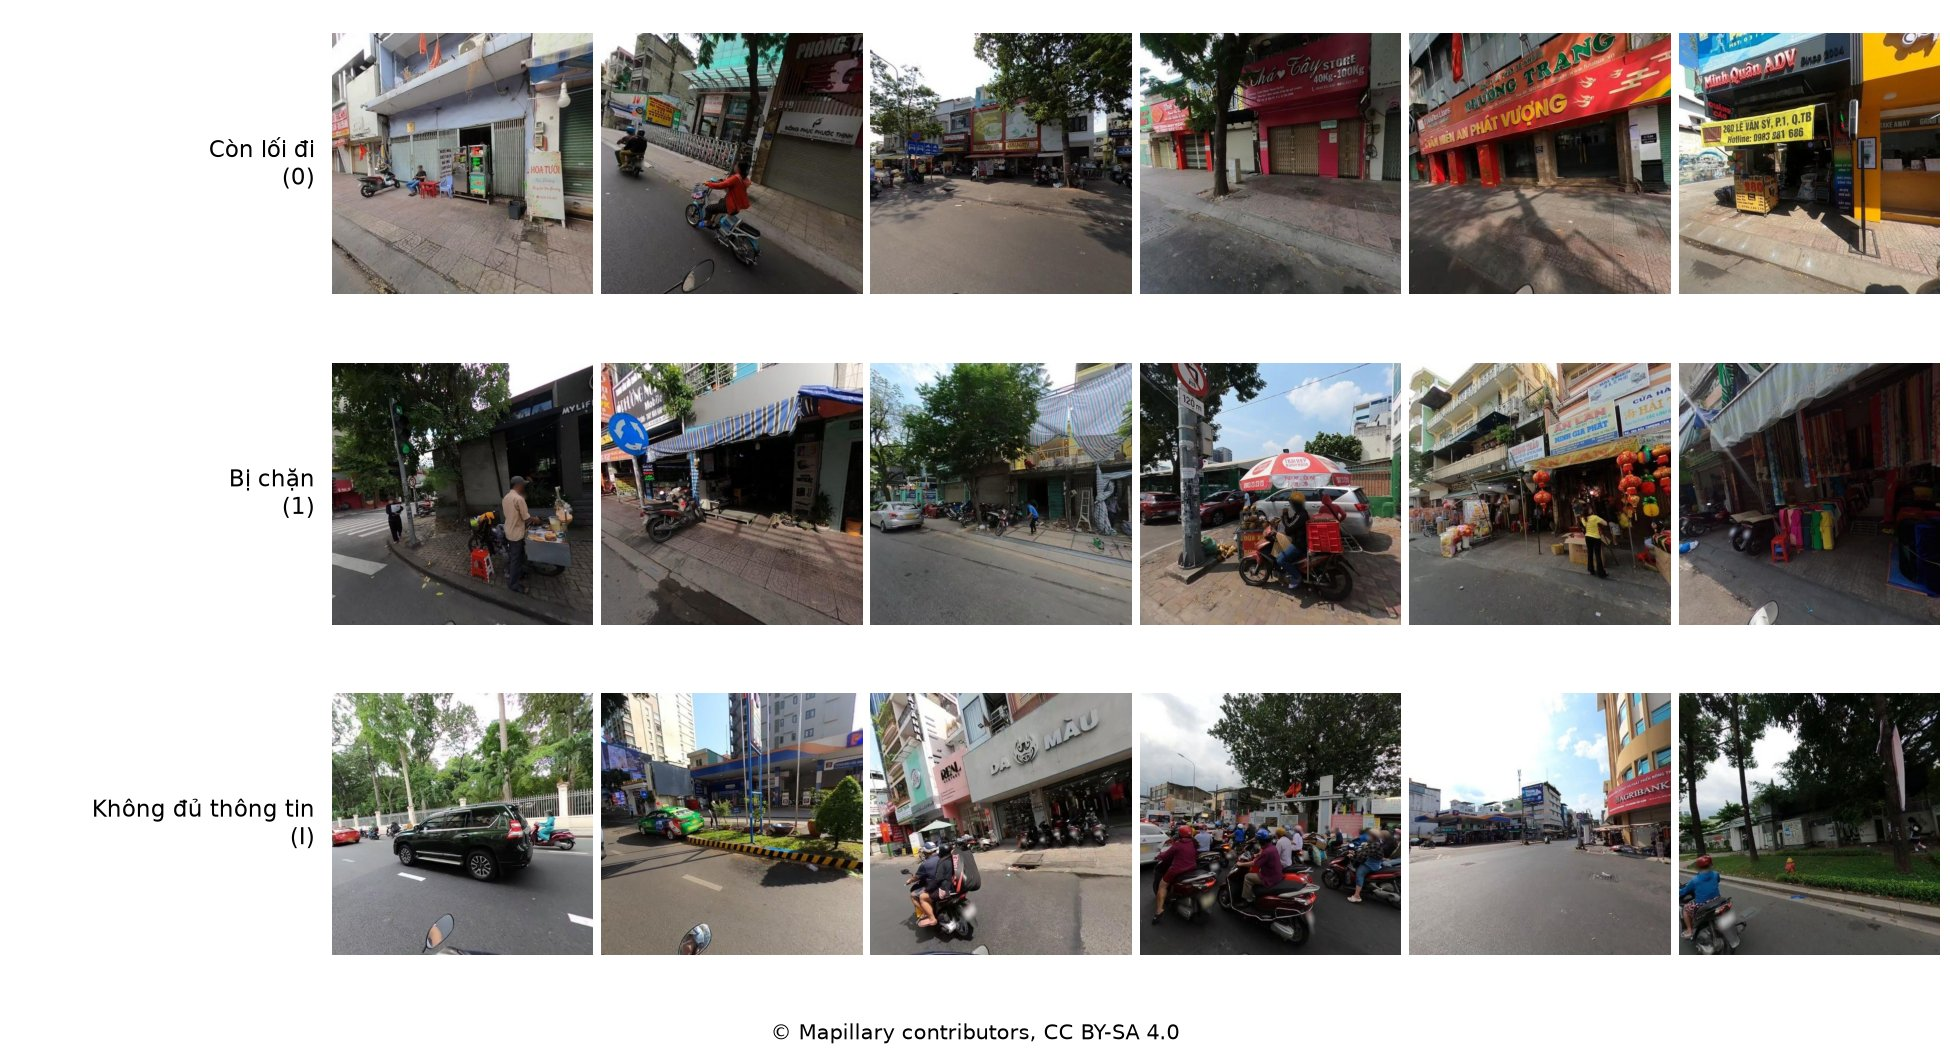
\includegraphics[width=\textwidth]{img_examples_main_train.jpg}
\caption{Ví dụ ảnh theo nhãn, lấy ngẫu nhiên từ train của bộ chính. \cc}
\label{fig:examples}
\end{figure}

\begin{figure}[H]
\centering
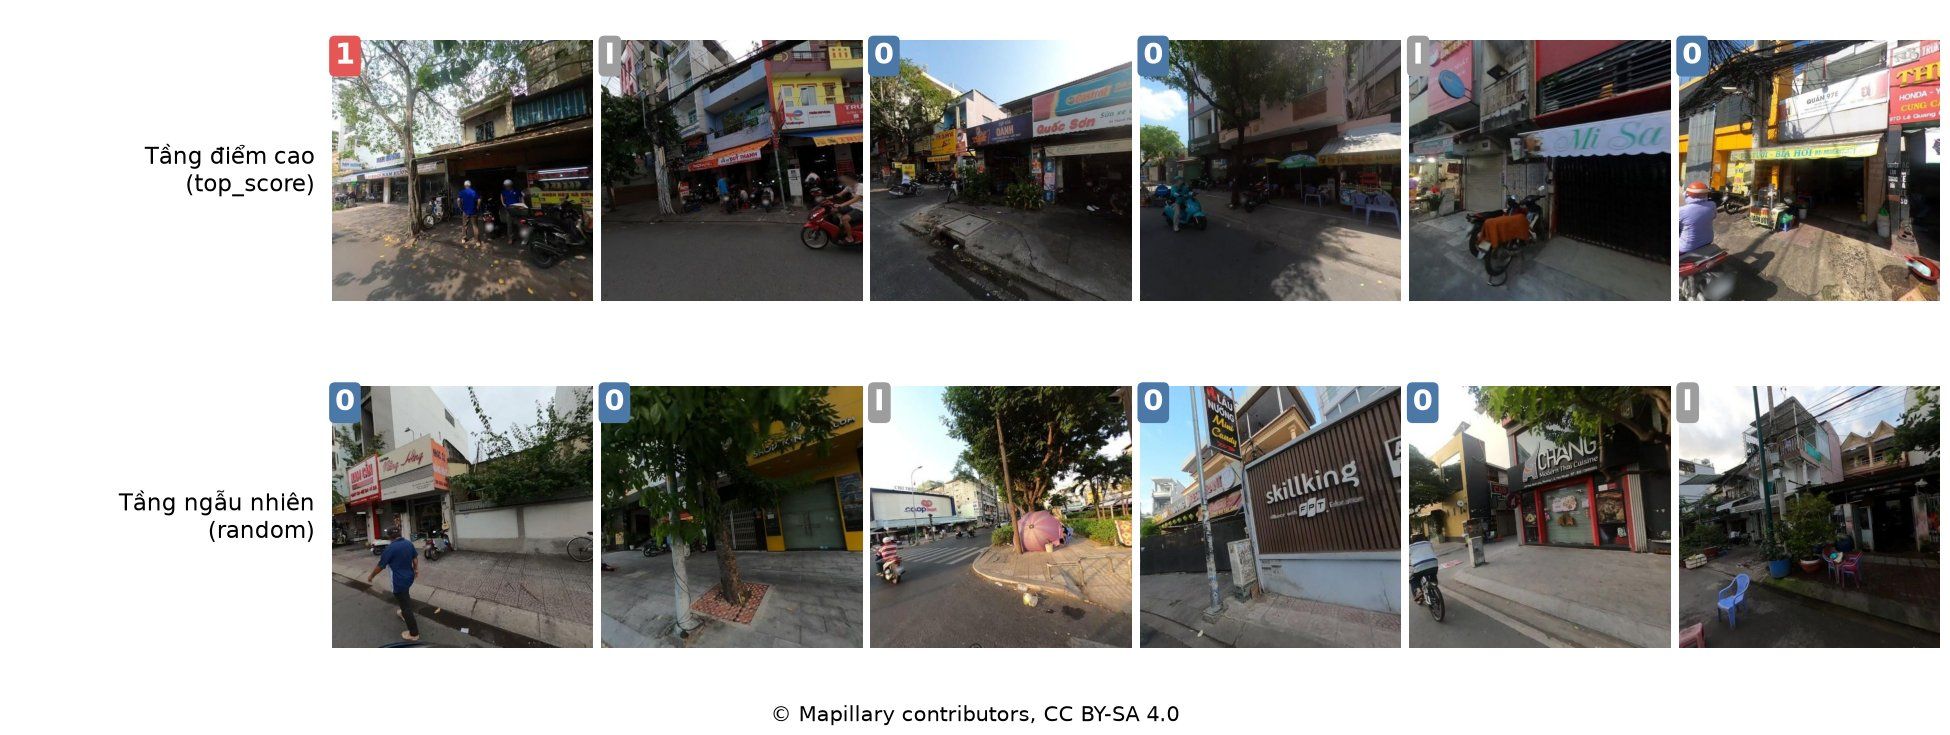
\includegraphics[width=\textwidth]{img_examples_train_extra.jpg}
\caption[Ví dụ ảnh bổ sung theo tầng lấy mẫu]{Ví dụ ảnh bổ sung theo tầng lấy mẫu; mỗi tầng gồm 6 ảnh lấy ngẫu nhiên nên tỉ lệ nhãn trong hình không đại diện cho tầng; ô góc trái ghi nhãn của ảnh. \cc}
\label{fig:examples-extra}
\end{figure}

\subsubsection*{Định dạng và độ phân giải}

Toàn bộ 5.149 ảnh đều đọc được, ở định dạng JPEG RGB $640\times640$ điểm ảnh, chất lượng nén ước lượng 90. Dung lượng mỗi ảnh từ 38,5 đến 167,7 KB, trung vị 99,3 KB. Độ phân giải đồng nhất theo thiết kế; do ảnh gốc là ảnh $360^\circ$ đã thu nhỏ còn 2.048 điểm ảnh, các chi tiết nhỏ ở xa bị mất.

\subsubsection*{Chất lượng ảnh}

Các đại lượng được đo trên từng ảnh cắt gồm: độ sáng trung bình (thang xám Rec.601, 0--255), độ tương phản (độ lệch chuẩn của thang xám), tỉ lệ điểm ảnh rất tối ($<30$) và cháy sáng ($>245$), độ nét (phương sai của toán tử Laplacian) và độ sặc sỡ màu~\cite{hasler2003colorfulness}.

\begin{table}[H]
\centering
\caption{Thống kê chất lượng ảnh theo nhóm (trung vị; trong ngoặc là IQR)}
\label{tab:image}
\begin{tabularx}{\textwidth}{>{\raggedright\arraybackslash}p{0.21\linewidth} r R R R R}
\toprule
\textbf{Nhóm} & \textbf{n} & \textbf{Độ sáng} & \textbf{Tương phản} & \textbf{Độ nét} & \textbf{Sặc sỡ màu} \\
\midrule
Bộ chính, train & 1.839 & 101,9 (31,3) & 59,4 (14,1) & 494 (254) & 25,1 (13,3) \\
Bộ chính, val & 486 & 106,7 (36,9) & 62,7 (14,1) & 560 (354) & 26,7 (13,7) \\
Bộ chính, test & 674 & 104,7 (36,9) & 59,3 (14,2) & 511 (245) & 25,9 (14,0) \\
Pilot & 150 & 106,6 (38,0) & 59,3 (14,0) & 487 (244) & 24,5 (13,1) \\
Ảnh bổ sung, tầng điểm cao & 1.400 & 91,8 (30,5) & 60,1 (13,7) & 492 (260) & 27,8 (14,3) \\
Ảnh bổ sung, tầng ngẫu nhiên & 600 & 100,8 (35,2) & 58,1 (12,4) & 497 (268) & 25,7 (13,7) \\
\midrule
Cả 5.149 ảnh: nhỏ nhất -- lớn nhất & & 24,3 -- 242,3 & 17,4 -- 96,6 & 22 -- 1.881 & 4,8 -- 104,3 \\
\bottomrule
\end{tabularx}
\end{table}

\begin{figure}[H]
\centering
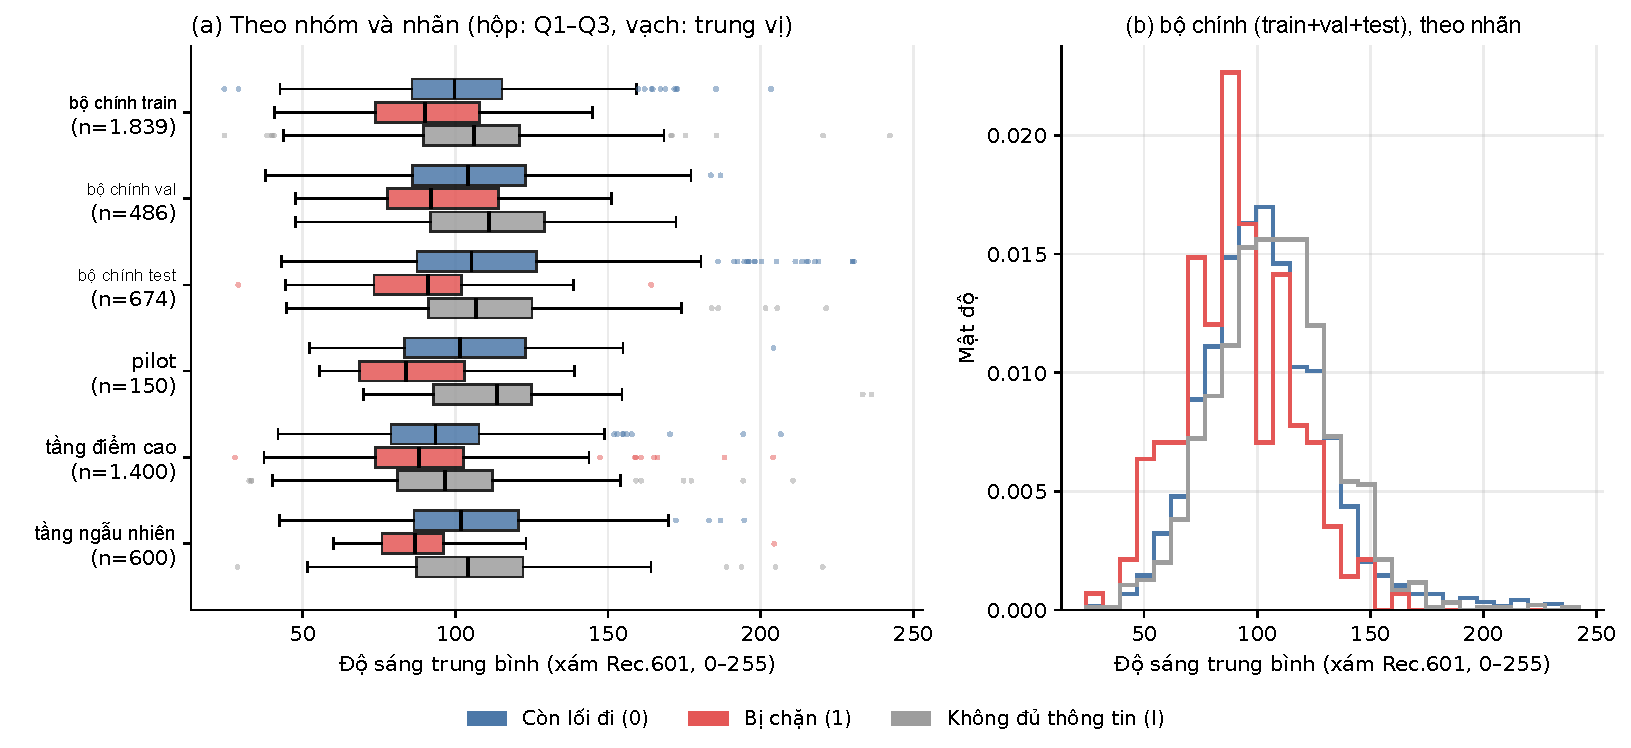
\includegraphics[width=\textwidth]{img_dist_luminance.pdf}
\caption{Độ sáng của ảnh cắt theo nhóm và theo nhãn}
\label{fig:lum}
\end{figure}

\begin{figure}[H]
\centering
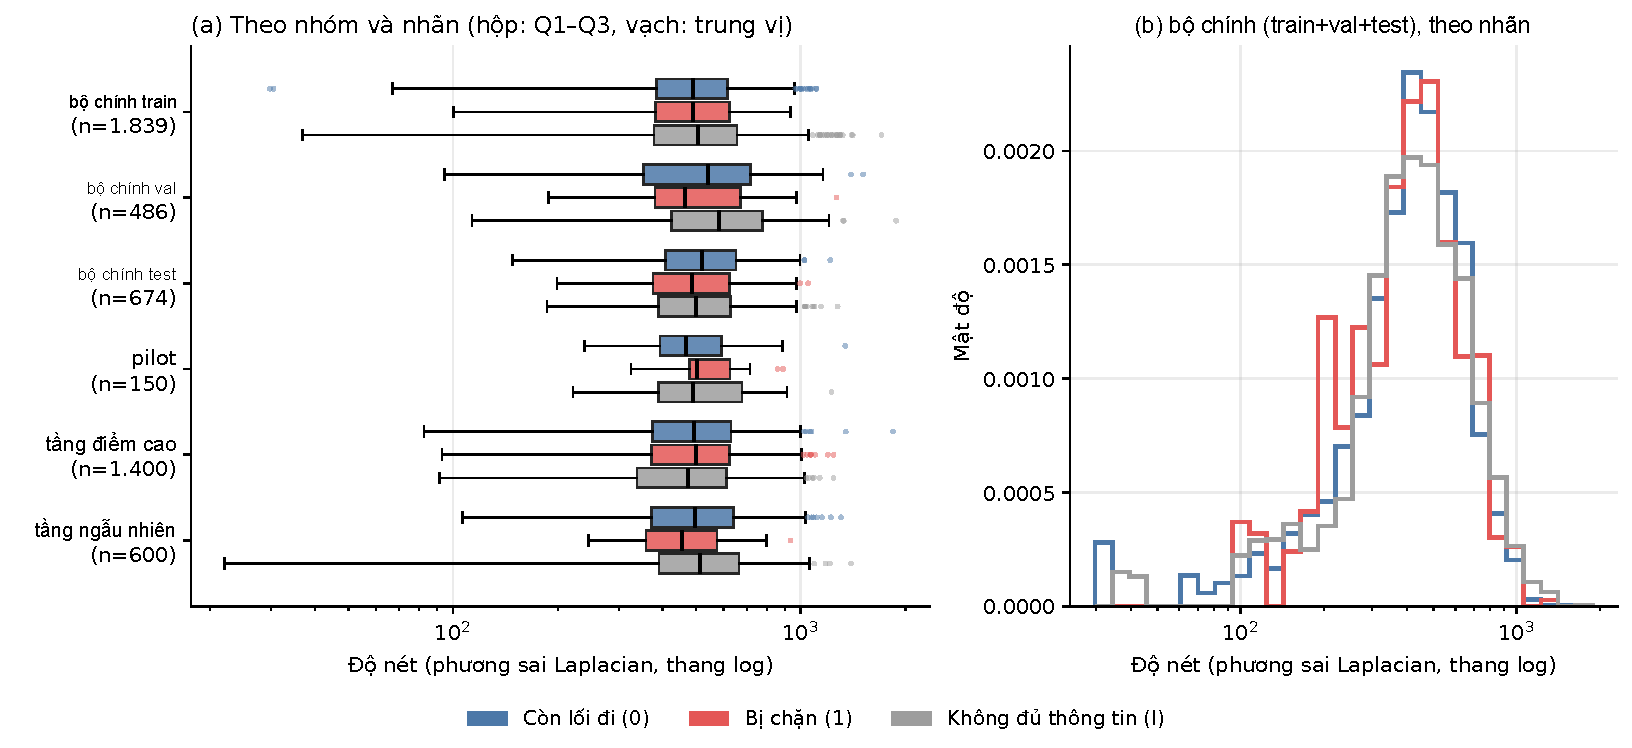
\includegraphics[width=\textwidth]{img_dist_sharpness.pdf}
\caption{Độ nét của ảnh cắt (thang log) theo nhóm và theo nhãn}
\label{fig:sharp}
\end{figure}

\begin{itemize}
  \item \textbf{Các nhóm tự nhiên có chất lượng ảnh tương đồng} (bảng~\ref{tab:image}, hình~\ref{fig:lum} và~\ref{fig:sharp}). Train, val, test, pilot và tầng ngẫu nhiên có trung vị độ sáng 101--107 và độ nét 487--560. Ảnh val có độ tương phản cao hơn train một chút (AUC 0,58 $[0{,}54;\,0{,}61]$).
  \item \textbf{Ảnh \lab{Bị chặn} tối hơn ảnh \lab{Còn lối đi}.} Ở bộ chính, trung vị độ sáng là 90,9 so với 101,6; AUC 0,37 $[0{,}32;\,0{,}41]$ (bootstrap theo 17 đường); tỉ lệ điểm ảnh rất tối là 18\% so với 12\%. Một cách giải thích hợp lý là vật cản thường nằm dưới mái hiên và bóng cây, nhưng giả thuyết này \textbf{chưa được kiểm chứng}. Đây là rủi ro học lối tắt: mô hình có thể dựa một phần vào độ tối của ảnh, nên cần kiểm tra khi phân tích lỗi mô hình.
  \item \textbf{Tầng điểm cao tối hơn bộ chính} (trung vị 91,8 so với 101,9), một phần vì tầng này có nhiều ảnh \lab{Bị chặn}.
  \item \textbf{Ảnh \lab{I} có độ tương phản cao hơn và nhiều vùng cháy sáng hơn} ảnh \lab{0} (AUC 0,67 và 0,65 ở bộ chính), phù hợp với việc các ảnh này thường chứa nhiều bầu trời và lòng đường.
  \item \textbf{Độ nét không phân biệt được \lab{Bị chặn} với \lab{Còn lối đi}} (AUC 0,46--0,59 ở mọi nhóm, mọi khoảng tin cậy đều chứa 0,5). Ở các so sánh có nhãn \lab{I}, hai khoảng tin cậy không chứa 0,5 nhưng hiệu ứng nhỏ: ở val, \lab{I} so với \lab{1} có AUC 0,61 $[0{,}53;\,0{,}71]$; ở tầng điểm cao, \lab{I} so với \lab{0} có AUC 0,46 $[0{,}42;\,0{,}49]$.
  \item \textbf{Độ sáng ảnh $360^\circ$ (dùng để lọc ảnh đêm) chỉ liên hệ yếu với độ sáng ảnh cắt} (Spearman 0,18 $[0{,}09;\,0{,}27]$ ở bộ chính; 0,31 nếu chỉ tính nửa trên ảnh cắt), vì hai đại lượng này đo hai vùng ảnh khác nhau. Do đó, bộ lọc ảnh đêm không bảo đảm ảnh cắt đủ sáng.
\end{itemize}

\subsubsection*{Đối chiếu lý do gán nhãn \lab{I} với phép đo chất lượng ảnh}

Có 33 ảnh \lab{I} mang lý do ``Ảnh mờ / tối / cháy sáng'' (bộ chính 12, ảnh bổ sung 21). Các ảnh này có độ nét thấp rõ rệt: trung vị độ nét nằm ở phân vị 3,5 của bộ chính và phân vị 13 của ảnh bổ sung. Về độ sáng, nhóm này gồm cả ảnh tối lẫn ảnh cháy sáng (36\% nằm dưới phân vị 10, 18\% nằm trên phân vị 90). Do cỡ mẫu nhỏ, kết quả này chỉ mang tính mô tả.

% ==============================================================================
% 7. TỔNG KẾT VÀ CÁC HẠN CHẾ
% ==============================================================================
\section{Tổng kết và các hạn chế}
\label{sec:summary}

\subsection{Các kết quả đã đo được}

Bảng~\ref{tab:measured} tổng hợp các kết quả chính, mỗi kết quả kèm cỡ mẫu và khoảng tin cậy.

\begin{longtable}{>{\raggedright\arraybackslash}p{0.3\linewidth} >{\raggedright\arraybackslash}p{0.41\linewidth} >{\raggedright\arraybackslash}p{0.2\linewidth}}
\caption{Các kết quả chính, kèm cỡ mẫu và khoảng tin cậy}
\label{tab:measured}\\
\toprule
\textbf{Câu hỏi} & \textbf{Kết quả} & \textbf{Phạm vi đo} \\
\midrule
\endfirsthead
\toprule
\textbf{Câu hỏi} & \textbf{Kết quả} & \textbf{Phạm vi đo} \\
\midrule
\endhead
Bộ dữ liệu có bao nhiêu ảnh và bao nhiêu ảnh hợp lệ? & 5.149 ảnh có nhãn cuối; 3.229 ảnh hợp lệ (2.450 ảnh \lab{0}, 779 ảnh \lab{1}); 1.920 ảnh \lab{I} & Toàn bộ dữ liệu \\
Lớp \lab{Bị chặn} hiếm tới mức nào trong ảnh tự nhiên? & 10,8\% số ảnh hợp lệ [Wilson 9,4; 12,3], [bootstrap theo đường 8,7; 13,9] & 1.746 ảnh hợp lệ, 17 đường \\
Test và val có đủ mẫu dương không? & Test có 47 ảnh (10,2\% [7,8; 13,4]); val có 35 ảnh (14,5\% [10,6; 19,4]) & 459 và 242 ảnh hợp lệ \\
Tập train thay đổi thế nào sau khi bổ sung? & 697 ảnh \lab{Bị chặn} trên 2.528 ảnh hợp lệ (27,6\% [25,9; 29,3]); 83\% mẫu dương đến từ ảnh bổ sung & Train \\
Người gán có nhất quán không? & Cohen $\kappa$ 3 nhãn: test 0,60; val 0,64; train gán chéo 0,61. 303 ảnh bất đồng do Khải phân xử, sửa 28 nhãn đề xuất & 674, 486, 276 ảnh gán đôi \\
Bộ chọn ảnh có hiệu quả trên đường mới không? & Tỉ lệ \lab{Bị chặn} trên mọi ảnh: tầng điểm cao 37,9\% [35,4; 40,5], tầng ngẫu nhiên 7,7\% [5,8; 10,1] & 1.400 và 600 ảnh \\
Có ảnh trùng lặp không? & Không có ảnh trùng lặp tuyệt đối; không có cặp nào có dHash $\le 4$ & 5.149 ảnh, mọi cặp \\
Có rò rỉ giữa các tập không? & Không có đường, vị trí hay ảnh gốc dùng chung. 52/1.160 ảnh val/test (4,5\%) cách ảnh train dưới 40 m tại giao lộ & Mọi ảnh, theo tọa độ \\
Chất lượng ảnh có khác nhau giữa các tập không? & Các chỉ số mô tả nhìn chung tương đồng giữa train, val và test của bộ chính. Ảnh \lab{Bị chặn} tối hơn ảnh \lab{Còn lối đi}: AUC 0,37 [0,32; 0,41] & 2.999 ảnh, 17 đường \\
Ảnh bổ sung có giống bộ chính không? & Không: bộ phân loại miền đạt AUC 0,70 ở tầng ngẫu nhiên và 0,95 ở tầng điểm cao (giá trị sau bị ước lượng cao một phần do dùng chung embedding với bộ chọn ảnh) & 1.839 so với 1.400 và 600 ảnh \\
Metadata có liên hệ với nhãn không? & Tuyến đường có liên hệ (Cramér's V 0,18); loại đường có V = 0,00 ở bộ chính, còn liên hệ ở ảnh bổ sung được trình bày riêng; chưa thấy liên hệ rõ với độ sáng ảnh $360^\circ$, tọa độ, tài khoản chụp và năm chụp & 1.746 ảnh hợp lệ \\
\bottomrule
\end{longtable}

\subsection{Các nội dung chưa đo hoặc chưa thực hiện}

Bảng~\ref{tab:notdone} liệt kê các việc còn tồn đọng và ảnh hưởng của từng việc tới các kết luận ở trên.

\begin{longtable}{>{\raggedright\arraybackslash}p{0.36\linewidth} >{\raggedright\arraybackslash}p{0.58\linewidth}}
\caption{Các việc chưa thực hiện và ảnh hưởng tới báo cáo}
\label{tab:notdone}\\
\toprule
\textbf{Nội dung} & \textbf{Trạng thái và ảnh hưởng} \\
\midrule
\endfirsthead
\toprule
\textbf{Nội dung} & \textbf{Trạng thái và ảnh hưởng} \\
\midrule
\endhead
Ảnh nhóm tự chụp (ít nhất 100 ảnh theo đề cương) & Chưa có. Toàn bộ dữ liệu hiện là ảnh Mapillary \\
Rà soát nội dung nhạy cảm trong ảnh & Chưa thực hiện. Hiện chỉ dựa vào phần làm mờ sẵn của Mapillary; trên các bảng ảnh kiểm tra vẫn thấy một số người và biển số còn rõ \\
Khóa danh sách chia tập & Chưa khóa. Nhóm giữ nguyên các đường test đã định; việc test chỉ có 47 mẫu dương là một hạn chế của đánh giá. Còn chờ quyết định về 47 ảnh train gần giao lộ với val/test \\
Mức nhiễu nhãn của ảnh bổ sung & Chưa đo được. Mỗi ảnh chỉ có một người gán; 203 ảnh được kiểm tra chéo được chọn vì bị nghi ngờ nên không đại diện. Tỉ lệ \lab{Bị chặn} giữa người gán chênh lệch rõ (19\% tới 43\%) \\
Phân xử độc lập (theo đề cương) & Chưa đạt hoàn toàn. Khải là người gán ở 123/303 ảnh bất đồng, gồm cả 99 ảnh bất đồng của val; 7 nhãn cuối khác cả hai phiếu \\
Khoảng tin cậy của $\kappa$ & Chưa tính \\
1.563 ảnh train của bộ chính chỉ có một người gán & Chưa được rà soát lại; phần gán chéo 15\% có $\kappa$ 0,61 \\
Vỉa hè bên trái của đường một chiều & Ít được quan sát vì chỉ cắt ảnh bên phải xe. Đây là giới hạn của nguồn dữ liệu \\
Gộp ảnh bổ sung vào bảng nhãn chung & Chưa gộp; hai bảng nhãn đang được lưu riêng. Hai ô kiểm tra chéo (263, 264) còn chờ xác nhận và đang giữ nhãn gốc \\
Giải thích vì sao ảnh \lab{Bị chặn} tối hơn & Chưa kiểm chứng; hiện mới dừng ở mức mô tả. Cần kiểm tra khi phân tích lỗi mô hình \\
Xem lại các ảnh bị bộ lọc ảnh đêm loại trong kho ứng viên bổ sung (38 ảnh) & Chưa xem lại. Ảnh bị loại của bộ chính (58 ảnh) đã được xem lại \\
So sánh ảnh dựng lại với bản gốc trên server & Chỉ có kết quả đo cũ trên 5 ảnh (lệch 1,35--1,5 mức xám). 671 ảnh val/test dùng trong EDA ảnh là bản dựng lại \\
Thời gian gán và thẻ vật cản của pilot & Chưa được đưa vào thống kê \\
Chuẩn hóa điểm ảnh, tăng cường dữ liệu & Thuộc giai đoạn huấn luyện, chưa thực hiện \\
\bottomrule
\end{longtable}

\subsection{Hệ quả đối với bước xây dựng mô hình}

\begin{itemize}
  \item \textbf{Đánh giá.} Nên dùng các chỉ số phù hợp với dữ liệu mất cân bằng, như diện tích dưới đường cong Precision--Recall (PR-AUC) và điểm F1 của lớp \lab{Bị chặn}, đồng thời báo cáo khoảng tin cậy bằng cách lấy mẫu lại theo đường. Với 47 mẫu dương ở test, khả năng phân biệt các chênh lệch nhỏ giữa các mô hình bị hạn chế.
  \item \textbf{Huấn luyện.} Phân phối nhãn và kiểu cảnh của train (sau khi bổ sung) khác với val/test. Nên chạy thêm một lượt huấn luyện chỉ với phần dữ liệu tự nhiên, và cân nhắc dùng trọng số lớp hoặc lấy mẫu lại.
  \item \textbf{Học lối tắt.} Cần kiểm tra xem mô hình có dựa vào độ tối của ảnh hay không.
  \item \textbf{Rò rỉ dữ liệu.} Cần quyết định cách xử lý các ảnh train gần giao lộ với val/test trước khi khóa chia tập.
\end{itemize}


\newpage
\bibliographystyle{unsrt}
\bibliography{references}

\appendix
% ==============================================================================
% PHỤ LỤC: TRUY NGUỒN SỐ LIỆU VÀ TÁI LẬP
% ==============================================================================
\needspace{0.6\textheight}
\section{Truy nguồn số liệu và cách tái lập}
\label{sec:trace}

Mọi con số trong báo cáo được tính bằng script của nhóm từ dữ liệu lưu trong repo (mục~\ref{sec:storage}); không có số liệu nào được nhập thủ công. Bảng~\ref{tab:scripts} cho biết mỗi nhóm số liệu được tạo ra ở bước nào.

\begin{table}[H]
\centering
\caption{Nguồn gốc của các nhóm số liệu trong báo cáo}
\label{tab:scripts}
\begin{tabularx}{\textwidth}{>{\raggedright\arraybackslash}p{0.36\linewidth} L}
\toprule
\textbf{Số liệu} & \textbf{Được tạo ra bởi} \\
\midrule
Số ảnh Mapillary, số đường OSM, tỉ lệ gắn đường, số ảnh đêm bị loại (mục~\ref{sec:pipeline}) & Các bước thu thập; kết quả của từng bước được ghi vào nhật ký thu thập và bảng trạng thái thu thập \\
So sánh ảnh bên trái và bên phải, tham số cắt ảnh & Hai phép đo thăm dò về độ phủ vỉa hè theo phía chụp và theo góc cắt \\
Đồng thuận, phân xử, nguồn nhãn (mục~\ref{sec:qa}) & Bước đo đồng thuận và dựng nhãn cuối từ phiếu gán và bảng phân xử \\
Bộ chọn ảnh, chọn đường, chọn 2.000 ảnh bổ sung (mục~\ref{sec:enrich}) & Phép so sánh các bộ chọn ảnh (để riêng từng tuyến đường), lượt quét 150 đường và bước chọn ảnh bổ sung \\
Kết quả gán nhãn ảnh bổ sung, kiểm tra chéo & Bước tổng hợp nhãn ảnh bổ sung từ phiếu gán và bảng kiểm tra chéo \\
Bảng~\ref{tab:overview}, \ref{tab:label-source}, \ref{tab:inventory}--\ref{tab:assoc}, \ref{tab:checks}; các hình về nhãn và metadata & Script EDA dữ liệu dạng bảng: đếm nhãn, khoảng tin cậy, thống kê mô tả, liên hệ với nhãn và 71 phép kiểm tra nhất quán; script này chỉ đọc bảng nhãn và manifest \\
Bảng~\ref{tab:image}; các hình về chất lượng ảnh và ảnh ví dụ & Script EDA ảnh: đo từng ảnh cắt (độ sáng, độ tương phản, tỉ lệ điểm ảnh tối và cháy sáng, độ nét, độ sặc sỡ màu) \\
Bảng~\ref{tab:spatial}, \ref{tab:domain}; các hình về trùng lặp, vị trí và t-SNE & Script EDA trùng lặp và rò rỉ: mã băm, dHash, embedding DINOv2, khoảng cách địa lý giữa các tập, bộ phân loại miền \\
\bottomrule
\end{tabularx}
\end{table}

\textbf{Tái lập kết quả.} Ảnh không được lưu trong git. Có hai cách lấy ảnh: dùng bản ảnh cắt trên server gán nhãn, hoặc dựng lại từ manifest (mã ảnh gốc và góc quay) bằng script dựng lại ảnh của nhóm, với điều kiện có token Mapillary. Bản dựng lại khác bản trên server do nén JPEG lại, nên cần ghi rõ nguồn ảnh đã dùng; 671 ảnh val/test trong phần EDA ảnh của báo cáo này là bản dựng lại. Tiếp theo, cài đặt các thư viện trong danh sách phụ thuộc của repo, ghi lại phiên bản Python và thư viện thực sự sử dụng, rồi chạy lần lượt ba script EDA (dạng bảng, ảnh, trùng lặp). Script dạng bảng chỉ cần các bảng dữ liệu; hai script còn lại cần kho ảnh cắt, và script trùng lặp nên được chạy trên GPU. Báo cáo được biên dịch bằng XeLaTeX và BibTeX.

\textbf{Phân công và việc sử dụng công cụ AI.} Ba script EDA do ba tác tử AI (Claude Sonnet) viết theo yêu cầu của một tác tử điều phối (Claude). Tác tử điều phối đã tính lại độc lập các số liệu chính (đếm nhãn, khoảng Wilson, thống kê metadata, phép đo ảnh trên 300 ảnh mẫu, mã băm MD5, khoảng cách giữa các tập, độ tương đồng embedding) và xem các bảng ảnh kiểm tra trước khi đưa kết quả vào báo cáo. Các kết quả kiểm tra trực quan trong báo cáo là quan sát của AI trên các bảng ảnh tổng hợp, không phải nhãn và không phải phép đo. Nhãn của bộ dữ liệu do người gán và người phân xử quyết định: Claude chỉ đề xuất nhãn cho 303 ảnh bất đồng của bộ chính (do Khải duyệt) và 150 ảnh pilot (do Phúc duyệt); 7 nhãn cuối của bộ chính là các đề xuất khác cả hai phiếu và được người phân xử giữ lại (mục~\ref{sec:qa}).

\textbf{Ảnh minh họa trong báo cáo.} Hình~\ref{fig:examples} và~\ref{fig:examples-extra} chỉ dùng ảnh train. Các bảng ảnh kiểm tra nội bộ có chứa ảnh val/test nên không được đưa vào báo cáo và không được đưa lên git. Nguồn ảnh: \cc.


\end{document}
